%%%%%%%%%%%%%%%%%%%%%%%%%%%%%%%%%%%%%%%%%%%%%%%%%%%%%%%%%%%%%%%%%%%%%
% Slide mode
\documentclass[10pt,hyperref={pdfpagelabels=false}]{beamer}
%%%%%%%%%%%%%%%%%%%%%%%%%%%%%%%%%%%%%%%%%%%%%%%%%%%%%%%%%%%%%%%%%%%%%
% Handout mode
%\documentclass[10pt,hyperref={pdfpagelabels=false},handout]{beamer}

%%%%%%%%%%%%%%%%%%%%%%%%%%%%%%%%%%%%%%%%%%%%%%%%%%%%%%%%%%%%%%%%%%%%%
% Packages & Setup
%%%%%%%%%%%%%%%%%%%%%%%%%%%%%%%%%%%%%%%%%%%%%%%%%%%%%%%%%%%%%%%%%%%%%

\usepackage{beamerthemeSAM}

\usepackage{etex}

\usepackage{amsfonts}
\usepackage{amsmath}
\usepackage{amssymb}
\usepackage{amsthm}
\usepackage{mathtools}
\usepackage{graphicx}  % for scalebox
%\usepackage{yhmath}    % for wider \widehat
%\usepackage{ifthen}
%\usepackage{bbm}
\usepackage{bm}
%\usepackage{upgreek}
%\usepackage{enumerate}
%\usepackage{array} % e.g. for specifying column separation
%\usepackage{multirow}
\usepackage{calc} % e.g. for \widthof
\usepackage{etoolbox}
\usepackage{float} % for [H] option of float placement
\usepackage{helvet}
\usepackage{scalerel,stackengine}
\usepackage{subcaption} % replacement for subfigure (obsolete) and subfig (out-of-date)
\usepackage{tikz}
\usetikzlibrary{calc,positioning,shadings,arrows.meta,backgrounds,cd}
\usepackage{pgfplots}
\pgfplotsset{compat=newest}
\usepackage{tikzscale}
\usepackage[ruled, titlenotnumbered, vlined]{algorithm2e} %for pseudocode
\usepackage{xparse}
\usepackage{varwidth}
\usepackage{examplep}


% optional

% blackboard letters
\providecommand{\bbA}{\mathbb{A}}
\providecommand{\bbB}{\mathbb{B}}
\providecommand{\bbC}{\mathbb{C}}
\providecommand{\bbD}{\mathbb{D}}
\providecommand{\bbE}{\mathbb{E}}
\providecommand{\bbF}{\mathbb{F}}
\providecommand{\bbG}{\mathbb{G}}
\providecommand{\bbH}{\mathbb{H}}
\providecommand{\bbI}{\mathbb{I}}
\providecommand{\bbJ}{\mathbb{J}}
\providecommand{\bbK}{\mathbb{K}}
\providecommand{\bbL}{\mathbb{L}}
\providecommand{\bbM}{\mathbb{M}}
\providecommand{\bbN}{\mathbb{N}}
\providecommand{\bbO}{\mathbb{O}}
\providecommand{\bbP}{\mathbb{P}}
\providecommand{\bbQ}{\mathbb{Q}}
\providecommand{\bbR}{\mathbb{R}}
\providecommand{\bbS}{\mathbb{S}}
\providecommand{\bbT}{\mathbb{T}}
\providecommand{\bbU}{\mathbb{U}}
\providecommand{\bbV}{\mathbb{V}}
\providecommand{\bbW}{\mathbb{W}}
\providecommand{\bbX}{\mathbb{X}}
\providecommand{\bbY}{\mathbb{Y}}
\providecommand{\bbZ}{\mathbb{Z}}

% calligraphic letters
\providecommand{\CA}{\mathcal{A}}
\providecommand{\CB}{\mathcal{B}}
\providecommand{\CC}{\mathcal{C}}
\providecommand{\CD}{\mathcal{D}}
\providecommand{\CE}{\mathcal{E}}
\providecommand{\CF}{\mathcal{F}}
\providecommand{\CG}{\mathcal{G}}
\providecommand{\CH}{\mathcal{H}}
\providecommand{\CI}{\mathcal{I}}
\providecommand{\CJ}{\mathcal{J}}
\providecommand{\CK}{\mathcal{K}}
\providecommand{\CL}{\mathcal{L}}
\providecommand{\CM}{\mathcal{M}}
\providecommand{\CN}{\mathcal{N}}
\providecommand{\CO}{\mathcal{O}}
\providecommand{\CP}{\mathcal{P}}
\providecommand{\CQ}{\mathcal{Q}}
\providecommand{\CR}{\mathcal{R}}
\providecommand{\CS}{\mathcal{S}}
\providecommand{\CT}{\mathcal{T}}
\providecommand{\CU}{\mathcal{U}}
\providecommand{\CV}{\mathcal{V}}
\providecommand{\CW}{\mathcal{W}}
\providecommand{\CX}{\mathcal{X}}
\providecommand{\CY}{\mathcal{Y}}
\providecommand{\CZ}{\mathcal{Z}}

%% Capital bold characters in math mode
%\providecommand{\BA}{{\boldsymbol{A}}}
%\providecommand{\BB}{{\boldsymbol{B}}}
%\providecommand{\BC}{{\boldsymbol{C}}}
%\providecommand{\BD}{{\boldsymbol{D}}}
%\providecommand{\BE}{{\boldsymbol{E}}}
%\providecommand{\BF}{{\boldsymbol{F}}}
%\providecommand{\BG}{{\boldsymbol{G}}}
%\providecommand{\BH}{{\boldsymbol{H}}}
%\providecommand{\BI}{{\boldsymbol{I}}}
%\providecommand{\BJ}{{\boldsymbol{J}}}
%\providecommand{\BK}{{\boldsymbol{K}}}
%\providecommand{\BL}{{\boldsymbol{L}}}
%\providecommand{\BM}{{\boldsymbol{M}}}
%\providecommand{\BN}{{\boldsymbol{N}}}
%\providecommand{\BO}{{\boldsymbol{O}}}
%\providecommand{\BP}{{\boldsymbol{P}}}
%\providecommand{\BQ}{{\boldsymbol{Q}}}
%\providecommand{\BR}{{\boldsymbol{R}}}
%\providecommand{\BS}{{\boldsymbol{S}}}
%\providecommand{\BT}{{\boldsymbol{T}}}
%\providecommand{\BU}{{\boldsymbol{U}}}
%\providecommand{\BV}{{\boldsymbol{V}}}
%\providecommand{\BW}{{\boldsymbol{W}}}
%\providecommand{\BX}{{\boldsymbol{X}}}
%\providecommand{\BY}{{\boldsymbol{Y}}}
%\providecommand{\BZ}{{\boldsymbol{Z}}}
%
%\providecommand{\Ba}{{\boldsymbol{a}}}
%\providecommand{\Bb}{{\boldsymbol{b}}}
%\providecommand{\Bc}{{\boldsymbol{c}}}
%\providecommand{\Bd}{{\boldsymbol{d}}}
%\providecommand{\Be}{{\boldsymbol{e}}}
%\providecommand{\Bf}{{\boldsymbol{f}}}
%\providecommand{\Bg}{{\boldsymbol{g}}}
%\providecommand{\Bh}{{\boldsymbol{h}}}
%\providecommand{\Bi}{{\boldsymbol{i}}}
%\providecommand{\Bj}{{\boldsymbol{j}}}
%\providecommand{\Bk}{{\boldsymbol{k}}}
%\providecommand{\Bl}{{\boldsymbol{l}}}
%\providecommand{\Bm}{{\boldsymbol{m}}}
%\providecommand{\Bn}{{\boldsymbol{n}}}
%\providecommand{\Bo}{{\boldsymbol{o}}}
%\providecommand{\Bp}{{\boldsymbol{p}}}
%\providecommand{\Bq}{{\boldsymbol{q}}}
%\providecommand{\Br}{{\boldsymbol{r}}}
%\providecommand{\Bs}{{\boldsymbol{s}}}
%\providecommand{\Bt}{{\boldsymbol{t}}}
%\providecommand{\Bu}{{\boldsymbol{u}}}
%\providecommand{\Bv}{{\boldsymbol{v}}}
%\providecommand{\Bw}{{\boldsymbol{w}}}
%\providecommand{\Bx}{{\boldsymbol{x}}}
%\providecommand{\By}{{\boldsymbol{y}}}
%\providecommand{\Bz}{{\boldsymbol{z}}}

% bold upright letters for vectors
\newcommand{\VA}{{\mathbf{A}}}
\newcommand{\VB}{{\mathbf{B}}}
\newcommand{\VC}{{\mathbf{C}}}
\newcommand{\VD}{{\mathbf{D}}}
\newcommand{\VE}{{\mathbf{E}}}
\newcommand{\VF}{{\mathbf{F}}}
\newcommand{\VG}{{\mathbf{G}}}
\newcommand{\VH}{{\mathbf{H}}}
\newcommand{\VI}{{\mathbf{I}}}
\newcommand{\VJ}{{\mathbf{J}}}
\newcommand{\VK}{{\mathbf{K}}}
\newcommand{\VL}{{\mathbf{L}}}
\newcommand{\VM}{{\mathbf{M}}}
\newcommand{\VN}{{\mathbf{N}}}
\newcommand{\VO}{{\mathbf{O}}}
\newcommand{\VP}{{\mathbf{P}}}
\newcommand{\VQ}{{\mathbf{Q}}}
\newcommand{\VR}{{\mathbf{R}}}
\newcommand{\VS}{{\mathbf{S}}}
\newcommand{\VT}{{\mathbf{T}}}
\newcommand{\VU}{{\mathbf{U}}}
\newcommand{\VV}{{\mathbf{V}}}
\newcommand{\VW}{{\mathbf{W}}}
\newcommand{\VX}{{\mathbf{X}}}
\newcommand{\VY}{{\mathbf{Y}}}
\newcommand{\VZ}{{\mathbf{Z}}}

\newcommand{\Va}{{\mathbf{a}}}
\newcommand{\Vb}{{\mathbf{b}}}
\newcommand{\Vc}{{\mathbf{c}}}
\newcommand{\Vd}{{\mathbf{d}}}
\newcommand{\Ve}{{\mathbf{e}}}
\newcommand{\Vf}{{\mathbf{f}}}
\newcommand{\Vg}{{\mathbf{g}}}
\newcommand{\Vh}{{\mathbf{h}}}
\newcommand{\Vi}{{\mathbf{i}}}
\newcommand{\Vj}{{\mathbf{j}}}
\newcommand{\Vk}{{\mathbf{k}}}
\newcommand{\Vl}{{\mathbf{l}}}
\newcommand{\Vm}{{\mathbf{m}}}
\newcommand{\Vn}{{\mathbf{n}}}
\newcommand{\Vo}{{\mathbf{o}}}
\newcommand{\Vp}{{\mathbf{p}}}
\newcommand{\Vq}{{\mathbf{q}}}
\newcommand{\Vr}{{\mathbf{r}}}
\newcommand{\Vs}{{\mathbf{s}}}
\newcommand{\Vt}{{\mathbf{t}}}
\newcommand{\Vu}{{\mathbf{u}}}
\newcommand{\Vv}{{\mathbf{v}}}
\newcommand{\Vw}{{\mathbf{w}}}
\newcommand{\Vx}{{\mathbf{x}}}
\newcommand{\Vy}{{\mathbf{y}}}
\newcommand{\Vz}{{\mathbf{z}}}

\newcommand{\Vzero}{\boldsymbol{0}}

%% Bold upright capital greek letters for _V_ectors and Matrices
%\newcommand{\VGamma}  {\mathbf{\Gamma}}
%\newcommand{\VDelta}  {\mathbf{\Delta}}
%\newcommand{\VTheta}  {\mathbf{\Theta}}
%\newcommand{\VLambda} {\mathbf{\Lambda}}
%\newcommand{\VXi}     {\mathbf{\Xi}}
%\newcommand{\VPi}     {\mathbf{\Pi}}
%\newcommand{\VPsi}    {\mathbf{\Psi}}
%\newcommand{\VSigma}  {\mathbf{\Sigma}}
%\newcommand{\VUpsilon}{\mathbf{\Upsilon}}
%\newcommand{\VPhi}    {\mathbf{\Phi}}
%\newcommand{\VOmega}  {\mathbf{\Omega}}

%% _B_old italicized capital greek letters
%\newcommand{\BGamma}  {\boldsymbol{\mathit{\Gamma}}}
%\newcommand{\BDelta}  {\boldsymbol{\mathit{\Delta}}}
%\newcommand{\BTheta}  {\boldsymbol{\mathit{\Theta}}}
%\newcommand{\BLambda} {\boldsymbol{\mathit{\Lambda}}}
%\newcommand{\BXi}     {\boldsymbol{\mathit{\Xi}}}
%\newcommand{\BPi}     {\boldsymbol{\mathit{\Pi}}}
%\newcommand{\BPsi}    {\boldsymbol{\mathit{\Psi}}}
%\newcommand{\BSigma}  {\boldsymbol{\mathit{\Sigma}}}
%\newcommand{\BUpsilon}{\boldsymbol{\mathit{\Upsilon}}}
%\newcommand{\BPhi}    {\boldsymbol{\mathit{\Phi}}}
%\newcommand{\BOmega}  {\boldsymbol{\mathit{\Omega}}}
%
%% Bold upright lower case greek letters for _V_ectors and matrices (requires package upgreek)
%\newcommand{\Valpha}     {\boldsymbol{\upalpha}}
%\newcommand{\Vbeta}      {\boldsymbol{\upbeta}}
%\newcommand{\Vgamma}     {\boldsymbol{\upgamma}}
%\newcommand{\Vdelta}     {\boldsymbol{\updelta}}
%\newcommand{\Vepsilon}   {\boldsymbol{\upepsilon}}
%\newcommand{\Vvarepsilon}{\boldsymbol{\upvarepsilon}}
%\newcommand{\Vzeta}      {\boldsymbol{\upzeta}}
%\newcommand{\Veta}       {\boldsymbol{\upeta}} %
%\newcommand{\Vtheta}     {\boldsymbol{\uptheta}}
%\newcommand{\Vvartheta}  {\boldsymbol{\upvartheta}}
%\newcommand{\Viota}      {\boldsymbol{\upiota}}
%\newcommand{\Vkappa}     {\boldsymbol{\upkappa}}
%\newcommand{\Vlambda}    {\boldsymbol{\uplambda}}
%\newcommand{\Vmu}        {\boldsymbol{\upmu}}
%\newcommand{\Vnu}        {\boldsymbol{\upnu}}
%\newcommand{\Vxi}        {\boldsymbol{\upxi}}
%\newcommand{\Vpi}        {\boldsymbol{\uppi}}
%\newcommand{\Vvarpi}     {\boldsymbol{\upvarpi}}
%\newcommand{\Vrho}       {\boldsymbol{\uprho}}
%\newcommand{\Vvarrho}    {\boldsymbol{\upvarrho}}
%\newcommand{\Vsigma}     {\boldsymbol{\upsigma}}
%\newcommand{\Vvarsigma}  {\boldsymbol{\upvarsigma}}
%\newcommand{\Vtau}       {\boldsymbol{\uptau}}
%\newcommand{\Vupsilon}   {\boldsymbol{\upupsilon}}
%\newcommand{\Vphi}       {\boldsymbol{\upphi}}
%\newcommand{\Vvarphi}    {\boldsymbol{\upvarphi}}
%\newcommand{\Vchi}       {\boldsymbol{\upchi}}
%\newcommand{\Vpsi}       {\boldsymbol{\uppsi}}
%\newcommand{\Vomega}     {\boldsymbol{\upomega}}

%% _B_old italicised lower case Greek letters
%\newcommand{\Balpha}     {\boldsymbol{\alpha}}
%\newcommand{\Bbeta}      {\boldsymbol{\beta}}
%\newcommand{\Bgamma}     {\boldsymbol{\gamma}}
%\newcommand{\Bdelta}     {\boldsymbol{\delta}}
%\newcommand{\Bepsilon}   {\boldsymbol{\epsilon}}
%\newcommand{\Bvarepsilon}{\boldsymbol{\varepsilon}}
%\newcommand{\Bzeta}      {\boldsymbol{\zeta}}
%\newcommand{\Beta}       {\boldsymbol{\eta}}                % \Beta=B undefined
%\newcommand{\Btheta}     {\boldsymbol{\theta}}
%\newcommand{\Bvartheta}  {\boldsymbol{\vartheta}}
%\newcommand{\Biota}      {\boldsymbol{\iota}}
%\newcommand{\Bkappa}     {\boldsymbol{\kappa}}
%\newcommand{\Blambda}    {\boldsymbol{\lambda}}
%\newcommand{\Bmu}        {\boldsymbol{\mugreek}}
%\newcommand{\Bnu}        {\boldsymbol{\nu}}
%\newcommand{\Bxi}        {\boldsymbol{\xi}}
%\newcommand{\Bpi}        {\boldsymbol{\pi}}
%\newcommand{\Bvarpi}     {\boldsymbol{\varpi}}
%\newcommand{\Brho}       {\boldsymbol{\rho}}
%\newcommand{\Bvarrho}    {\boldsymbol{\varrho}}
%\newcommand{\Bsigma}     {\boldsymbol{\sigma}}
%\newcommand{\Bvarsigma}  {\boldsymbol{\varsigma}}
%\newcommand{\Btau}       {\boldsymbol{\tau}}
%\newcommand{\Bupsilon}   {\boldsymbol{\upsilon}}
%\newcommand{\Bphi}       {\boldsymbol{\phi}}
%\newcommand{\Bvarphi}    {\boldsymbol{\phi}}
%\newcommand{\Bchi}       {\boldsymbol{\chi}}
%\newcommand{\Bpsi}       {\boldsymbol{\psi}}
%\newcommand{\Bomega}     {\boldsymbol{\omega}}

% "Fraktur" letters
\providecommand{\FA}{\mathfrak{A}}
\providecommand{\FB}{\mathfrak{B}}
\providecommand{\FC}{\mathfrak{C}}
\providecommand{\FD}{\mathfrak{D}}
\providecommand{\FE}{\mathfrak{E}}
\providecommand{\FF}{\mathfrak{F}}
\providecommand{\FG}{\mathfrak{G}}
\providecommand{\FH}{\mathfrak{H}}
\providecommand{\FI}{\mathfrak{I}}
\providecommand{\FJ}{\mathfrak{J}}
\providecommand{\FK}{\mathfrak{K}}
\providecommand{\FL}{\mathfrak{L}}
\providecommand{\FM}{\mathfrak{M}}
\providecommand{\FN}{\mathfrak{N}}
\providecommand{\FO}{\mathfrak{O}}
\providecommand{\FP}{\mathfrak{P}}
\providecommand{\FQ}{\mathfrak{Q}}
\providecommand{\FR}{\mathfrak{R}}
\providecommand{\FS}{\mathfrak{S}}
\providecommand{\FT}{\mathfrak{T}}
\providecommand{\FU}{\mathfrak{U}}
\providecommand{\FV}{\mathfrak{V}}
\providecommand{\FW}{\mathfrak{W}}
\providecommand{\FX}{\mathfrak{X}}
\providecommand{\FY}{\mathfrak{Y}}
\providecommand{\FZ}{\mathfrak{Z}}

\providecommand{\Fa}{\mathfrak{a}}
\providecommand{\Fb}{\mathfrak{b}}
\providecommand{\Fc}{\mathfrak{c}}
\providecommand{\Fd}{\mathfrak{d}}
\providecommand{\Fe}{\mathfrak{e}}
\providecommand{\Ff}{\mathfrak{f}}
\providecommand{\Fg}{\mathfrak{g}}
\providecommand{\Fh}{\mathfrak{h}}
\providecommand{\Fi}{\mathfrak{i}}
\providecommand{\Fj}{\mathfrak{j}}
\providecommand{\Fk}{\mathfrak{k}}
\providecommand{\Fl}{\mathfrak{l}}
\providecommand{\Fm}{\mathfrak{m}}
\providecommand{\Fn}{\mathfrak{n}}
\providecommand{\Fo}{\mathfrak{o}}
\providecommand{\Fp}{\mathfrak{p}}
\providecommand{\Fq}{\mathfrak{q}}
\providecommand{\Fr}{\mathfrak{r}}
\providecommand{\Fs}{\mathfrak{s}}
\providecommand{\Ft}{\mathfrak{t}}
\providecommand{\Fu}{\mathfrak{u}}
\providecommand{\Fv}{\mathfrak{v}}
\providecommand{\Fw}{\mathfrak{w}}
\providecommand{\Fx}{\mathfrak{x}}
\providecommand{\Fy}{\mathfrak{y}}
\providecommand{\Fz}{\mathfrak{z}}
\newcommand{\mse}{\boldsymbol{\varepsilon}_{mse}}
\newcommand{\learningrate}{\alpha}
\newcommand{\relu}{\operatorname{ReLU}}
\newcommand{\prelu}{\operatorname{PReLU}}
\newcommand{\indicator}{\mathbb{I}}
\newcommand{\dataset}{\mathcal{S}}
\newcommand{\loss}{\mathcal{J}}
\newcommand{\nn}{\boldsymbol{\Phi}}

\newcommand*{\wt}[1]{\widetilde{#1}}
\newcommand*{\wh}[1]{\widehat{#1}}

\newcommand{\matlab}{{\sc Matlab}\xspace}
\newcommand{\ttt}[1]{\textnormal{\texttt{#1}}}
\newcommand{\eps}{\varepsilon}
\newcommand{\fin}{{\mathrm{fin}}}

\newcommand{\Hs}[1][s]{H^{\vec s}} % has to be called with square brackets
%\newcommand{\Hks}[1][\vec s]{H^{k+#1}} % has to be called with square brackets

\newcommand{\dd}{\mathop{}\!\text{\textup{d}}} % \mathop for correct spacing
\newcommand{\ee}{\mathrm{e}}
\newcommand{\ii}{\mathrm{i}}
\newcommand{\id}{\mathbbm{1}}
\newcommand{\ind}{\mathbbm{1}}

\newcommand{\rmr}{\textup{r}}
\newcommand{\rms}{\textup{s}}

\newcommand{\bbSd}{\bbS^{d-1}}

\newcommand{\argmin}{\mathop{\mathrm{argmin}}}
\newcommand{\ran}{\textup{ran}}
\renewcommand{\ker}{\textup{ker}}
\newcommand{\sinc}{\textup{sinc}}
\newcommand{\supp}{\textup{supp}\mathop{}}
\newcommand{\dist}{\textup{dist}}
\newcommand{\diag}{\textup{diag}}
\newcommand{\spann}{\operatorname{span}}
\newcommand{\grad}{\operatorname{grad}}
\renewcommand{\div}{\operatorname{div}}
\newcommand{\sgn}{\operatorname{sgn}}

\newcommand{\err}{\mathrm{err}}
\newcommand{\rel}{\mathrm{rel}}

\newcommand{\herm}{\mathsf{H}}

\newcommand{\jl}{{j\!\?\?,\ell}}
\newcommand{\jld}{{j'\!\!,\?\?\ell'}}
\newcommand{\jldd}{{j''\!\!,\?\?\ell''}}
\newcommand{\jlk}{{j\!\?\?,\?\ell\!\?\?,\?\vec k}}
\newcommand{\jlkd}{{j'\!\!,\?\?\ell'\!\!,\?\?\vec k{}'}}
\newcommand{\lld}{{\lambda,\lambda'}}
\newcommand{\jjd}{{j,j'}}
\newcommand{\mmd}{{m,m'}}
\newcommand{\Rn}{R_{\vec n}}% attention with biblatex!
\newcommand{\Rs}{R_{\vec s}}
\newcommand{\Rsd}{R_{\vec s'}}
\newcommand{\Rjl}{R_\jl}
\newcommand{\Rjld}{R_\jld}
\newcommand{\tilRjl}{\wt R_\jl}
\newcommand{\tilRjld}{\wt R_\jld}
\newcommand{\sjl}{\vec s_\jl}
\newcommand{\sjld}{\vec s_\jld}

\newcommand{\psp}{p\textup{-sparse}}

% macros for superscripts of number 1st, 2nd, 3rd, 4th etc.
\newcommand{\tsp}[1]{\textsuperscript{#1}}
\newcommand{\tsb}[1]{\textsubscript{#1}}
\newcommand{\nth}{\textsuperscript{th}\xspace} % \th is occupied by thorn-rune
\newcommand{\st}{\textsuperscript{st}\xspace}
\newcommand{\nd}{\textsuperscript{nd}\xspace}
\newcommand{\rd}{\textsuperscript{rd}\xspace}


%%%%%%%%%%%%%%%%%%%%%%%%%%%%%%%%%%%%%%%%%%%%%%%%%%%%%%%%%%%%%%%%%%%%%%%%%%%
% Differential operators, "normal" and partial
%%%%%%%%%%%%%%%%%%%%%%%%%%%%%%%%%%%%%%%%%%%%%%%%%%%%%%%%%%%%%%%%%%%%%%%%%%%

\NewDocumentCommand{\Dn} {m O{} m}  {\frac{\dd^{#1}#2}{\dd{#3}^{#1}}}
\NewDocumentCommand{\Dnp}{m O{} m}  {\frac{\partial^{#1}#2}{\partial{#3}^{#1}}}
\NewDocumentCommand{\Dpp}{m O{} m m}{\frac{\partial^{#1}#2}{\partial{#3}\,\partial{#4}}}
\NewDocumentCommand{\D}  {O{} m}    {\Dn{}[#1]{#2}}
\NewDocumentCommand{\DD} {O{} m}    {\Dn{2}[#1]{#2}}
\NewDocumentCommand{\Dp} {O{} m}    {\Dnp{}[#1]{#2}}
\NewDocumentCommand{\DDp}{O{} m}    {\Dnp{2}[#1]{#2}}

%%%%%%%%%%%%%%%%%%%%%%%%%%%%%%%%%%%%%%%%%%%%%%%%%%%%%%%%%%%%%%%%%%%%%%%%%%%
% Delimiters
%%%%%%%%%%%%%%%%%%%%%%%%%%%%%%%%%%%%%%%%%%%%%%%%%%%%%%%%%%%%%%%%%%%%%%%%%%%

% Define delimiter pairs, resp. appearance of inner product and sets. The final versions are defined below to have default left/right-delimiters and don't crash if both a star and a size argument is present.
% A star is a shortcut to the most important size \big, else an optional argument can be given for the size, see mathtools-documentation. The reason to use these commands is unified appearance, as well as the fact that Latex can't know if vertical bars - i.e. | or \| - are a left or a right delimiter, and thus the spacing would be wrong.
\DeclarePairedDelimiter {\nrmInternal}   {\lVert} {\rVert}
\DeclarePairedDelimiter {\absInternal}   {\lvert} {\rvert}
\DeclarePairedDelimiter {\parInternal}   {\lparen}{\rparen}
\DeclarePairedDelimiter {\braInternal}   {\lbrack}{\rbrack}
\DeclarePairedDelimiter {\ceiInternal}   {\lceil} {\rceil}
\DeclarePairedDelimiter {\flrInternal}   {\lfloor}{\rfloor}
\DeclarePairedDelimiter {\inpInternal}   {\langle}{\rangle}
\DeclarePairedDelimiter {\crlInternal}   {\{}     {\}}
\DeclarePairedDelimiterX{\setInternal}[2]{\{}     {\}}     {#1\;\delimsize|\;#2}

% All of the following commands have the same structure:
% 1. argument: append star to operatorname for \big-delimiters (no star defaults to left/right)
% 2. argument: optional specification of size (\big,\Big,\bigg, etc.)
% 3./4. argument: content between delimiters
\NewDocumentCommand{\norm}   {s o m}  {\resizerOneInput {\nrmInternal}{#1}{#2}{#3}    }
\NewDocumentCommand{\abs}    {s o m}  {\resizerOneInput {\absInternal}{#1}{#2}{#3}    }
\NewDocumentCommand{\snorm}  {s o m}  {\resizerOneInput {\absInternal}{#1}{#2}{#3}    }
\NewDocumentCommand{\card}   {s o m}  {\resizerOneInput {\absInternal}{#1}{#2}{#3}    }
\NewDocumentCommand{\parens} {s o m}  {\resizerOneInput {\parInternal}{#1}{#2}{#3}    }
\NewDocumentCommand{\bracket}{s o m}  {\resizerOneInput {\braInternal}{#1}{#2}{#3}    }
\NewDocumentCommand{\ceil}   {s o m}  {\resizerOneInput {\ceiInternal}{#1}{#2}{#3}    }
\NewDocumentCommand{\floor}  {s o m}  {\resizerOneInput {\flrInternal}{#1}{#2}{#3}    }
\NewDocumentCommand{\inpr}   {s o m}  {\resizerOneInput {\inpInternal}{#1}{#2}{#3}    }
\NewDocumentCommand{\reg}    {s o m}  {\resizerOneInput {\inpInternal}{#1}{#2}{#3}    }
\NewDocumentCommand{\curly}  {s o m}  {\resizerOneInput {\crlInternal}{#1}{#2}{#3}    }
\NewDocumentCommand{\set}    {s o m m}{\resizerTwoInputs{\setInternal}{#1}{#2}{#3}{#4}}

\NewDocumentCommand{\resizerOneInput}{m m m m}{
% First argument is an internal command from \DeclarePairedDelimiter, second is star for \big-delimiters, third is optional size parameter (overridden if star is present!), fourth is content between delimiters.
	\IfBooleanTF{#2}   % star yes/no
		{#1[\big]{#4}} % star triggers \big
		{\IfNoValueTF{#3} % no star -> check if size specified
			{#1*{#4}}     % uses \left...\right
			{#1[#3]{#4}}} % uses size specified
}
\NewDocumentCommand{\resizerTwoInputs}{m m m m m}{
% Like above but with two inputs for internal command from \DeclarePairedDelimiterX
	\IfBooleanTF{#2}
		{#1[\big]{#4}{#5}}
		{\IfNoValueTF{#3}
			{#1*{#4}{#5}}
			{#1[#3]{#4}{#5}}}
}

%%%%%%%%%%%%%%%%%%%%%%%%%%%%%%%%%%%%%%%%%%%%%%%%%%%%%%%%%%%%%%%%%%%%%%%%%%%
% Tools
%%%%%%%%%%%%%%%%%%%%%%%%%%%%%%%%%%%%%%%%%%%%%%%%%%%%%%%%%%%%%%%%%%%%%%%%%%%

\newlength{\hspacetemp} % to be able to use \widthof in hspace, on has to set a length with setlength first, which has to be defined

\newcommand{\lcopywidth}[2]{%
	\phantom{\smash{#2}}\mathllap{#1}}
\newcommand{\ccopywidth}[2]{% 					if used for subscripts, #2 needs to be passed
	\setlength{\hspacetemp}{\widthof{$#2$}}% 	with "\scriptstyle" in front.
	\hspace{0.5\hspacetemp}\mathclap{#1}\vphantom{#2}\hspace{0.5\hspacetemp}}
\newcommand{\rcopywidth}[2]{%
	\mathrlap{#1}\phantom{\smash{#2}}}

\newcommand{\lsetwidth}[2]{%
	\hspace{#2}\mathllap{#1}}
\newcommand{\csetwidth}[2]{%
	\hspace{0.5\dimexpr#2}\mathclap{#1}\hspace{0.5\dimexpr#2}}
\newcommand{\rsetwidth}[2]{%
	\mathrlap{#1}\hspace{#2}}


%%%%%%%%%%%%%%%%%%%%%%%%%%%%%%%%%%%%%%%%%%%%%%%%%%%%%%%%%%%%%%%%%%%%%%%%%%%
% Package setup
%%%%%%%%%%%%%%%%%%%%%%%%%%%%%%%%%%%%%%%%%%%%%%%%%%%%%%%%%%%%%%%%%%%%%%%%%%%

\mathtoolsset{showonlyrefs=true}

\captionsetup{format=hang,justification=raggedright}

%%%%%%%%%%%%%%%%%%%%%%%%%%%%%%%%%%%%%%%%%%%%%%%%%%%%%%%%%%%%%%%%%%%%%%%%%%%
% Plotting
%%%%%%%%%%%%%%%%%%%%%%%%%%%%%%%%%%%%%%%%%%%%%%%%%%%%%%%%%%%%%%%%%%%%%%%%%%%

\newlength{\plotsize}

\makeatletter
\newcommand*{\overlaynumber}{\number\beamer@slideinframe}

\usetikzlibrary{external}
\usepackage{pdftexcmds}% for \pdfmdfivesum for tikz externalisation
\tikzset{
	external/system call={lualatex
		\tikzexternalcheckshellescape -halt-on-error -interaction=batchmode
		-jobname "\image" "\texsource"},
	external/only named=true,
	%%% see tex.stackexchange.com/a/119440/42225
	beamer externalizing/.style={%
		execute at end picture={%
			\tikzifexternalizing{%
				\ifbeamer@anotherslide%
				\pgfexternalstorecommand{\string\global\string\beamer@anotherslidetrue}%
				\fi%
			}{}%
		}%
	},
	external/optimize=false,
	every picture/.style={beamer externalizing}
}
\let\origtikzsetnextfilename=\tikzsetnextfilename
\renewcommand\tikzsetnextfilename[1]{\origtikzsetnextfilename{#1-\overlaynumber}}
\makeatother

\tikzexternalize[prefix=figures/ext/]

%%% for correct rendering of transparency, see tex.stackexchange.com/a/101283/42225
%%% for PDFLATEX!
%\pdfpageattr{/Group <</S /Transparency /I true /CS /DeviceRGB>>}
%%% for XELATEX!
%\usepackage{everypage}
%\AddEverypageHook{%
%	\makeatletter%
%	\special{pdf: put @thispage <</Group << /S /Transparency /I true /CS /DeviceRGB>> >>}%
%	\makeatother%
%}%

%%%%%%%%%%%%%%%%%%%%%%%%%%%%%%%%%%%%%%%%%%%%%%%%%%%%%%%%%%%%%%%%%%%%%%%%%%%
% Technical details
%%%%%%%%%%%%%%%%%%%%%%%%%%%%%%%%%%%%%%%%%%%%%%%%%%%%%%%%%%%%%%%%%%%%%%%%%%%

\newcommand{\normall}[1]{\mathopen{\displaystyle#1}}  % complements \bigl, \Bigl, \biggl, etc.
\newcommand{\normalr}[1]{\mathclose{\displaystyle#1}} % complements \bigr, \Bigr, \biggr, etc.

% No spurious spacing introduced by \left and \right, see http://tex.stackexchange.com/a/2610/42225
\let\oldleft\left
\let\oldright\right
\renewcommand{\left}{\mathopen{}\mathclose\bgroup\oldleft}
\renewcommand{\right}{\aftergroup\egroup\oldright}

% Somehow, \vec has problems for single letters, see e.g. \left|\vec{\xi}\right|, where the arrow touches the bar. This redefinition adds an empty second character to every argument, thus avoiding the problem.
\let\oldvec\vec
\def\vec#1{\oldvec{#1{}}}

% shifts in 18th of 1em: "\,": +3, "\:": +4, "\;": +5, "\!": -3
\newcommand{\?}{\:\!} % this shifts by +1/18th em

%% define every float to have \centering attribute, see http://tex.stackexchange.com/q/2651
%\makeatletter
%\g@addto@macro\@floatboxreset\centering
%\makeatother


%%%%%%%%%%%%%%%%%%%%%%%%%%%%%%%%%%%%%%%%%%%%%%%%%%%%%%%%%%%%%%%%%%%%%%%%%%%
% Table of contents in block + Command to generate it
%%%%%%%%%%%%%%%%%%%%%%%%%%%%%%%%%%%%%%%%%%%%%%%%%%%%%%%%%%%%%%%%%%%%%%%%%%%

\setbeamertemplate{section in toc}[blocktoc]
\setbeamertemplate{section in toc shaded}[blocktoc]
\setbeamertemplate{subsection in toc}[blocktoc]
\setbeamertemplate{subsection in toc shaded}[blocktoc]

% second argument is mandatory label, first command is optional for highlighting "currentsection" and/or "currentsubsection"
\NewDocumentCommand{\mytoc}{O{} m}{
\begin{frame}<handout:0>[label=#2]
\begin{block}{Table of Contents}
	\vspace{1.25em}%
	\tableofcontents[#1]%
\end{block}
\end{frame}
}

%%%%%%%%%%%%%%%%%%%%%%%%%%%%%%%%%%%%%%%%%%%%%%%%%%%%%%%%%%%%%%%%%%%%%%%%%%%
% Command for footcites (footnote adapted in beamerinnerthemeSAM to match appearance)
%%%%%%%%%%%%%%%%%%%%%%%%%%%%%%%%%%%%%%%%%%%%%%%%%%%%%%%%%%%%%%%%%%%%%%%%%%%

% fix \footnotemark for referencing, see tex.stackexchange.com/a/38859/42225
\patchcmd{\footnotemark}{\stepcounter{footnote}}{\refstepcounter{footnote}}{}{}
% compare tex.stackexchange.com/q/30720 and tex.stackexchange.com/q/45437/
\makeatletter
\newcommand\myfootnote[2]{%
	\begingroup
	\let\@footnotemark\relax
	\let\@makefnmark\relax
	\let\thefootnote\relax
	\renewcommand\@makefntext[1]{\parindent 0em\noindent\usebeamerfont{footnote}\llap{#1\enskip}##1}
	\footnote{#2}%
	\addtocounter{footnote}{-1}%
	\endgroup
}
\newcommand\blindfootnote[1]{
	\myfootnote{}{#1}
}
\makeatother

%%%%%%%%%%%%%%%%%%%%%%%%%%%%%%%%%%%%%%%%%%%%%%%%%%%%%%%%%%%%%%%%%%%%%%%%%%%
% Useful tweaks
%%%%%%%%%%%%%%%%%%%%%%%%%%%%%%%%%%%%%%%%%%%%%%%%%%%%%%%%%%%%%%%%%%%%%%%%%%%

\newcommand{\normalitem}%
	{{\scriptsize\raise1.25pt\hbox{\color{cblue}$\blacktriangleright$}}\hspace{0.5em}}
\newcommand{\grayitem}%
	{{\scriptsize\raise1.25pt\hbox{\color{gray}$\blacktriangleright$}}}

\tikzset{onslide/.code args={<#1>#2}{%
	\only<#1>{\pgfkeysalso{#2}}% \pgfkeysalso doesn't change the path
}}

\makeatletter % see tex.stackexchange.com/a/141379
\newcommand{\breakcaption}{\@dblarg\emit@breakcaption}
\long\def\emit@breakcaption[#1]#2{%
  \expandafter\caption\expandafter[\expandafter\emit@removeafter#1\\\@nil]{%
    \begin{varwidth}[t]{\textwidth-\widthof{Figure:\space}}
    #2
    \end{varwidth}%
  }%
}
\def\emit@removeafter#1\\#2\@nil{#1}
\makeatother

%%%%%%%%%%%%%%%%%%%%%%%%%%%%%%%%%%%%%%%%%%%%%%%%%%%%%%%%%%%%%%%%%%%%%%%%%%%
% Place beamer buttons absolutely
%%%%%%%%%%%%%%%%%%%%%%%%%%%%%%%%%%%%%%%%%%%%%%%%%%%%%%%%%%%%%%%%%%%%%%%%%%%

\makeatletter
\newcommand{\placebuttons}[2][1mm]{%
\begin{tikzpicture}[remember picture,overlay]
	\node[inner sep=0pt,anchor=south east] at ($(current page.south east)+(-\beamer@rightmargin,5mm+#1)$)
		{#2};
\end{tikzpicture}
}
\makeatother

%%%%%%%%%%%%%%%%%%%%%%%%%%%%%%%%%%%%%%%%%%%%%%%%%%%%%%%%%%%%%%%%%%%%%%%%%%%
% Nice quote environment
%%%%%%%%%%%%%%%%%%%%%%%%%%%%%%%%%%%%%%%%%%%%%%%%%%%%%%%%%%%%%%%%%%%%%%%%%%%

% based on tex.stackexchange.com/a/16981/42225
%\usepackage{libertine} % or any other font package
\newcommand*\quotefont{\fontfamily{LinuxLibertineT-LF}}% selects Libertine as the quote font
\newcommand*\quotesize{45} % if quote size changes, need a way to make shifts relative

\newcommand*{\openquote}{\tikz[remember picture,overlay]%
	\node[anchor=east,inner sep=0pt,xshift=-0.75ex,yshift=-1.75ex] (OQ) {{{\quotefont\fontsize{\quotesize}{\quotesize}\selectfont``\kern5pt}}};}

\newcommand*{\closequote}{\tikz[remember picture,overlay]%
	\node[anchor=west,inner sep=0pt,xshift=0.75ex,yshift=-3.5ex] (CQ) {{{\quotefont\fontsize{\quotesize}{\quotesize}\selectfont\kern-7pt''}}};}

\newenvironment{myquote}{\begin{quote}\openquote\begin{minipage}[t]{\linewidth}}{\end{minipage}\closequote\end{quote}}
% Macros for dissertation
% FLM, ETH Zurich

\def \dissNo {24385}
\def \dissYear {2017}
\def \isbn {\todo{add ISBN}}
\def \doi {\todo{add DOI}}

\newcommand{\garding}{G\aa{}rding}
\newcommand{\cbsi}{Cauchy-Bunyakowski\u{\i}-Schwarz inequality}
\newcommand{\iagm}{inequality of arithmetic and geometric means}

% Tags
\newcommand{\todopic}[1]{{\color{red}{!! TODO:} generate picture: #1\\}}
\newcommand{\todo}[1]{{\color{red}{[TODO: #1]}}}
\newcommand{\fm}[1]{{\color{blue}{#1}}}
\newcommand{\fmOld}{}

% Text
\newcommand{\pylibs}{\texttt}
\newcommand{\ie}{i.\,e.~}
%\newcommand{\st}{s.\,t.~}
\newcommand{\mathst}{\text{ \st }}
\newcommand{\setst}{\,\mid\,}
\newcommand{\eg}{e.\,g.~}
\renewcommand{\wr}{w.\,r.~}

%\newcommand{\argmin}{\operatorname{argmin}}

% Triangulation
\newcommand{\tri}{\Tcal}
\newcommand{\vertTri}{\Vcal}
\newcommand{\edgesTri}{\Ecal}
\newcommand{\hUnifGM}{\mathsf{h}_0}
\newcommand{\hUnifFam}{\mathfrak{H}}
\newcommand{\nGMRef}{\mathsf{L}}
\newcommand{\GMind}{n}
\newcommand{\finfor}{\mathsf{F}}
\newcommand{\forest}{\mathbb{F}}
\newcommand{\shReg}{\kappa}
\newcommand{\femsp}[2]{S^{#1, 1}(\dom, #2)}
\newcommand{\polsp}[2]{\Pcal^{#1}(#2)}
\newcommand{\interp}[1]{\Ical^{(#1)}}
\newcommand{\incircrad}{\rho}
\newcommand{\CFLcste}{C}
\newcommand{\condnum}{\operatorname{cond}}

% Numbers
\newcommand{\nCor}{\Msf}
\newcommand{\nPol}{\Nsf}
\newcommand{\nKerDim}{\Jsf}
\newcommand{\nEigenDim}{\Lsf}
\newcommand{\nSer}{\Isf}
\newcommand{\nSys}{m}
\newcommand{\indSys}{j}
\newcommand{\indSetKer}{\Scal}
\newcommand{\nEl}{\femdim}
\newcommand{\femdim}{M}

% Operators
\renewcommand{\div}{\operatorname{div}}
\newcommand{\disjUnion}{\,\dot{\cup}\,}
\newcommand{\ellProj}[1]{\Pi_{#1}}
%\newcommand{\id}{\operatorname{Id}}
\newcommand{\Mell}[1]{\tilde{#1}}
\newcommand{\Mellin}{\Mcal}
\newcommand{\thetaOp}{\Dcal}
\newcommand{\contOp}{\X}
\newcommand{\fracDiff}{\Dsf}
\newcommand{\pencil}{\Afrak}
\newcommand{\dalem}{\square}
\newcommand{\dalemStr}{\Lcal}
\newcommand{\ellip}{\Acal}
\newcommand{\ellipMat}{\Abf}
\newcommand{\neumOp}{\Ncal}
\newcommand{\bdOp}{\Bcal}
\newcommand{\trOp}{\Tcal}
\newcommand{\domOp}{\operatorname{dom}}
\newcommand{\im}{\operatorname{im}}
\newcommand{\spec}{\operatorname{Spec}}
%\newcommand{\supp}{\operatorname{supp}}
%\newcommand{\grad}[1]{\operatorname{\bf grad}{#1}}

% Spaces
\renewcommand{\dh}{\mathsf{DH}_{\weightbf,s}}
\newcommand{\rh}{\mathsf{RH}_{\weightbf,s}}
\newcommand{\dv}{\mathsf{DV}_{\weightbf,s}}
\newcommand{\rv}{\mathsf{RV}_{\weightbf,s}}

% Time integration
\newcommand{\tend}{T}
\newcommand{\tint}{\Jfrak}
\newcommand{\nTime}{N}
\newcommand{\deltat}{\Delta t}
\newcommand{\newmG}{\eta}
\newcommand{\newmB}{\varrho}
\newcommand{\unumf}[1]{\ubf_{\femdim}^{(#1)}}
\newcommand{\znumf}[1]{\xibf_{\femdim}^{(#1)}}
\newcommand{\unum}[1]{\vec{\ubf}_{\femdim}^{(#1)}}
\newcommand{\znum}[1]{\vec{\xibf}_{\femdim}^{(#1)}}
\newcommand{\erry}[1]{\mathbf{e}_{0;\femdim}^{(#1)}}
\newcommand{\errz}[1]{\mathbf{e}_{1;\femdim}^{(#1)}}
\newcommand{\erreps}[1]{\etabf_{0;\femdim}^{(#1)}}
\newcommand{\erreta}[1]{\etabf_{1;\femdim}^{(#1)}}

% Boundary notations
\newcommand{\extsymb}{\text{bd}}
\newcommand{\intsymb}{\text{int}}
\newcommand{\totsymb}{{}}
\newcommand{\exterior}{^{\extsymb}}
\newcommand{\interior}{^{\intsymb}}
\newcommand{\total}{^{\totsymb}}
\newcommand{\diri}{^{\extsymb, D}}
\newcommand{\neum}{^{\extsymb, N}}
\newcommand{\polar}{^{\text{pol}}}
\newcommand{\normVect}{\nbf}

% Domain stuff
\newcommand{\singfun}{\Sbf}
\renewcommand{\reg}{\text{reg}}
\newcommand{\dom}{\Dfrak}
\newcommand{\cyl}{\Qfrak}
\newcommand{\cone}{\Cfrak}
\newcommand{\x}{\xbf}
\newcommand{\angCoord}{\theta}
\newcommand{\distance}{\Phibf}
\newcommand{\opangle}{\alpha}
\newcommand{\minang}{\underline{\alpha}}
\newcommand{\corner}{\cbf}
\newcommand{\corners}{\Ccal}
\newcommand{\edge}{\esf}
\newcommand{\edges}{\Fcal}
\newcommand{\diff}{\nabla}
\newcommand{\dual}[3]{\left\langle #1,#2 \right\rangle_{#3}}

% Singular exponents, weights and grading exponents
%\newcommand{\imagEig}{\gamma}
\newcommand{\mparam}{\xi}
\newcommand{\mparambf}{\boldsymbol{\mparam}}
\newcommand{\fparam}{\tau}
\newcommand{\fparamR}{\sigma}
\newcommand{\tweight}{\gamma}
\newcommand{\singexp}{\zeta}
\newcommand{\singexpbf}{\mparambf}
\newcommand{\imSingExp}{\omega}
\newcommand{\weight}{\delta}
\newcommand{\weightbf}{\deltabf}
\newcommand{\grading}{\beta}
\newcommand{\gradingbf}{\betabf}

% Math commands
\newcommand{\fourier}{\Ffrak}
\newcommand{\imag}{\mathsf{i}}
\newcommand{\setCond}{\,\vert\,}
%\newcommand{\dd}[2]{\frac{\partial #1}{\partial #2}}
%\newcommand{\abs}[1]{\left|#1\right|}
%\newcommand{\inprod}[2]{\left( #1, #2 \right)}
%\newcommand{\Span}[1]{\mbox{\upshape span}\left\{#1\right\}}
%\newcommand{\norm}[2]{\left\| #1 \,; #2\right\|}
%\newcommand{\seminorm}[2]{\left| #1\,; #2 \right|}

% Beauty
\renewcommand{\epsilon}{\varepsilon}

% Blackboard letters
\newcommand{\C}{\mathbb{C}}
\newcommand{\E}{\mathbb{E}}
\newcommand{\F}{\mathbb{F}}
\newcommand{\I}{\mathbb{I}}
\newcommand{\N}{\mathbb{N}}
\newcommand{\Q}{\mathbb{Q}}
\newcommand{\R}{\mathbb{R}}
\newcommand{\X}{\mathbb{X}}
\newcommand{\Z}{\mathbb{Z}}

% Bold face
\newcommand{\Abf}{\mathbf{A}}
\newcommand{\Bbf}{\mathbf{B}}
\newcommand{\Cbf}{\mathbf{C}}
\newcommand{\Dbf}{\mathbf{D}}
\newcommand{\Ebf}{\mathbf{E}}
\newcommand{\Fbf}{\mathbf{F}}
\newcommand{\Hbf}{\mathbf{H}}
\newcommand{\Ibf}{\mathbf{I}}
\newcommand{\Kbf}{\mathbf{K}}
\newcommand{\Mbf}{\mathbf{M}}
\newcommand{\Nbf}{\mathbf{N}}
\newcommand{\Rbf}{\mathbf{R}}
\newcommand{\Sbf}{\mathbf{S}}
\newcommand{\abf}{\mathbf{a}}
\newcommand{\bbf}{\mathbf{b}}
\newcommand{\cbf}{\mathbf{c}}
\newcommand{\fbf}{\mathbf{f}}
\newcommand{\gbf}{\mathbf{g}}
\newcommand{\lbf}{\mathbf{l}}
\newcommand{\nbf}{\mathbf{n}}
\newcommand{\rbf}{\mathbf{r}}
\newcommand{\sbf}{\mathbf{s}}
\newcommand{\ubf}{\mathbf{u}}
\newcommand{\vbf}{\mathbf{v}}
\newcommand{\wbf}{\mathbf{w}}
\newcommand{\xbf}{\mathbf{x}}
\newcommand{\zbf}{\mathbf{z}}
\newcommand{\y}{\mathbf{y}}
\newcommand{\ybf}{\mathbf{y}}

% Bold face greek
\newcommand{\Phibf}{\boldsymbol{\Phi}}
\newcommand{\varphibf}{\boldsymbol{\varphi}}
\newcommand{\Thetabf}{\boldsymbol{\Theta}}
\newcommand{\alphabf}{\boldsymbol{\alpha}}
\newcommand{\betabf}{\boldsymbol{\beta}}
\newcommand{\deltabf}{\boldsymbol{\delta}}
\newcommand{\nubf}{\boldsymbol{\nu}}
\newcommand{\etabf}{\boldsymbol{\eta}}
\newcommand{\phibf}{\boldsymbol{\phi}}
\newcommand{\psibf}{\boldsymbol{\psi}}
\newcommand{\mubf}{\boldsymbol{\mu}}
\newcommand{\xibf}{\boldsymbol{\xi}}
\newcommand{\sigmabf}{\boldsymbol{\sigma}}
\newcommand{\epsilonbf}{\boldsymbol{\epsilon}}
\newcommand{\zerobf}{\boldsymbol{0}}
\newcommand{\onebf}{\boldsymbol{1}}

%Frak
\newcommand{\afrak}{\mathfrak{a}}
\newcommand{\cfrak}{\mathfrak{c}}
\newcommand{\Afrak}{\mathfrak{A}}
\newcommand{\Bfrak}{\mathfrak{B}}
\newcommand{\Cfrak}{\mathfrak{C}}
\newcommand{\Dfrak}{\mathfrak{D}}
\newcommand{\Ffrak}{\mathfrak{F}}
\newcommand{\Jfrak}{\mathfrak{J}}
\newcommand{\Kfrak}{\mathfrak{K}}
\newcommand{\Nfrak}{\mathfrak{N}}
\newcommand{\Qfrak}{\mathfrak{Q}}
\newcommand{\Tfrak}{\mathfrak{T}}
\newcommand{\Ufrak}{\mathfrak{U}}
\newcommand{\Vfrak}{\mathfrak{V}}
\newcommand{\Wfrak}{\mathfrak{W}}

%Cal
\newcommand{\Acal}{\mathcal{A}}
\newcommand{\Bcal}{\mathcal{B}}
\newcommand{\Ccal}{\mathcal{C}}
\newcommand{\Dcal}{\mathcal{D}}
\newcommand{\Ecal}{\mathcal{E}}
\newcommand{\Fcal}{\mathcal{F}}
\newcommand{\Hcal}{\mathcal{H}}
\newcommand{\Ical}{\mathcal{I}}
\newcommand{\Jcal}{\mathcal{J}}
\newcommand{\Kcal}{\mathcal{K}}
\newcommand{\Lcal}{\mathcal{L}}
\newcommand{\Mcal}{\mathcal{M}}
\newcommand{\Ncal}{\mathcal{N}}
\newcommand{\Pcal}{\mathcal{P}}
\newcommand{\Rcal}{\mathcal{R}}
\newcommand{\Scal}{\mathcal{S}}
\newcommand{\Tcal}{\mathcal{T}}
\newcommand{\Vcal}{\mathcal{V}}
\newcommand{\Xcal}{\mathcal{X}}
\newcommand{\Ycal}{\mathcal{Y}}

% SF
\newcommand{\esf}{\mathsf{e}}
\newcommand{\Dsf}{\mathsf{D}}
\newcommand{\Isf}{\mathsf{I}}
\newcommand{\Jsf}{\mathsf{J}}
\newcommand{\Lsf}{\mathsf{L}}
\newcommand{\Msf}{\mathsf{M}}
\newcommand{\Nsf}{\mathsf{N}}

\newcommand\equalhat{\mathrel{\stackon[1.5pt]{=}{\stretchto{%
    \scalerel*[\widthof{=}]{\wedge}{\rule{1ex}{3ex}}}{0.5ex}}}}

\usepackage{graphicx}


\usepackage{pgf,tikz}
\usetikzlibrary{arrows}
\usetikzlibrary[patterns]

\usepackage{pgfplots}
\pgfplotsset{width=7cm,compat=1.8}
\usepackage{pgfplotstable}
\pgfmathsetseed{1138} % set the random seed
\pgfplotstableset{ % Define the equations for x and y
    create on use/x/.style={create col/expr={42+2*\pgfplotstablerow}},
    create on use/y/.style={create col/expr={(0.6*\thisrow{x}+130)+5*rand}}
}
% create a new table with 30 rows and columns x and y:
\pgfplotstablenew[columns={x,y}]{30}\loadedtable

\def\layersep{2cm}

%%%%%%%%%%%%%%%%%%%%%%%%%%%%%%%%%%%%%%%%%%%%%%%%%%%%%%%%%%%%%%%%%%%%%
% Title Information
%%%%%%%%%%%%%%%%%%%%%%%%%%%%%%%%%%%%%%%%%%%%%%%%%%%%%%%%%%%%%%%%%%%%%

\title%
{Introduction to Deep Learning}

\author[ Fabian M\"uller]{Fabian M\"uller, PhD}
\institute{Ziemer Ophthalmic Systems in Bienne, Switzerland}

\date{June 11\nth 2019, University of Cape Verde}

%%%%%%%%%%%%%%%%%%%%%%%%%%%%%%%%%%%%%%%%%%%%%%%%%%%%%%%%%%%%%%%%%%%%%
% Title Page
%%%%%%%%%%%%%%%%%%%%%%%%%%%%%%%%%%%%%%%%%%%%%%%%%%%%%%%%%%%%%%%%%%%%%

\begin{document}

\setbeamerfont{title}{size=\large} % instead of \Large in beamerfontthemedefault, because I have a long title
\frame[t,plain]{\titlepage}

%%%%%%%%%%%%%%%%%%%%%%%%%%%%%%%%%%%%%%%%%%%%%%%%%%%%%%%%%%%%%%%%%%%%%
\section{Introduction}
%\mytoc[currentsection]{sec:introduction}
%%%%%%%%%%%%%%%%%%%%%%%%%%%%%%%%%%%%%%%%%%%%%%%%%%%%%%%%%%%%%%%%%%%%%
\begin{frame}
    \frametitle{What is Machine Learning?}
    \begin{itemize}
        \item {\bf Given:} A decision task humans can do without knowing the exact decision mechanics.
        {\small
        \item Examples:
            \begin{enumerate}
                \item From a time series of measurements, identify outliers.
                \item Classifying Emails for Spam/No Spam
                \item Identifying different parts of an eye from an image.
                \item Generating images from pictures in a certain style.
            \end{enumerate}
        }
        \item {\bf Problem:} The decision ''algorithm'' our brain follows is far from understood, and therefore impossible to program.
        \item {\bf Solution:} Use an approach {\bf based on given data}. Find solutions to your task by minimizing an \emph{error function} over the data.
        \item Main paradigms: {\bf Supervised} vs {\bf unsupervised} learning.
    \end{itemize}
\end{frame}
%%%%%%%%%%%%%%%%%%%%%%%%%%%%%%%%%%%%%%%%%%%%%%%%%%%%%%%%%%%%%%%%%%%%%
\begin{frame}
    \frametitle{Example: Image Classification}
    \begin{itemize}
        \item \emph{Given:} An image taken with 4MP resolution: $3\cdot 4\cdot 10^6$ numbers.\\
        \emph{Goal:} A number $p\in[0,1]$ corresponding to the likelihood that there is a car in the picture.
        \item Deep neural networks in a nutshell:
        \begin{enumerate}
            \item \label{step:nn1}Compute linear combinations of the input numbers.
            \item \label{step:nn2}Apply non-linear functions to the results.
            \item Repeat steps \ref{step:nn1}-\ref{step:nn2} with the output of step \ref{step:nn2}.
        \end{enumerate}
        \item Coefficients in the linear combinations of step \ref{step:nn1}:
        \begin{enumerate}
            \item Each choice of coefficients yields an output $p(I)$ for each image $I$.
            \item Prepare a {\bf dataset} of $N_{\text{car}}$ images with cars ($p_{\text{exact}}(I)=1$) and $N_{\text{not car}}$ images without cars ($p_{\text{exact}}(I)=0$).
            \item Try to find a choice of coefficients which minimizes $p-p_{\text{exact}}$ on the given data set (in some sense).
        \end{enumerate}
        \item[$\Rightarrow$] Crucial to find good datasets and minimization procedures!
    \end{itemize}
\end{frame}
%%%%%%%%%%%%%%%%%%%%%%%%%%%%%%%%%%%%%%%%%%%%%%%
\begin{frame}
    \frametitle{Another example}
    \begin{minipage}{.5\textwidth}
        {\small
        \begin{itemize}
            \item {\bf Example:} From the image of an eye, locate the pupil as ellipse.
            \item Ellipses: Determined by centre coordinates, two major axes, tilt angle: {\bf Predict 5 numbers.}
            \item {\bf Ground truth:} We are given a {\bf labeled dataset} of 1000 images \emph{with their ''real'' ellipses} entered by humans.
            \item Getting a dataset can be difficult: Noise, balance, representation.
            \item Deep learning vs.~classical methods.
        \end{itemize}
        }
    \end{minipage}
    \begin{minipage}{.4\textwidth}
        \only<1>{\centering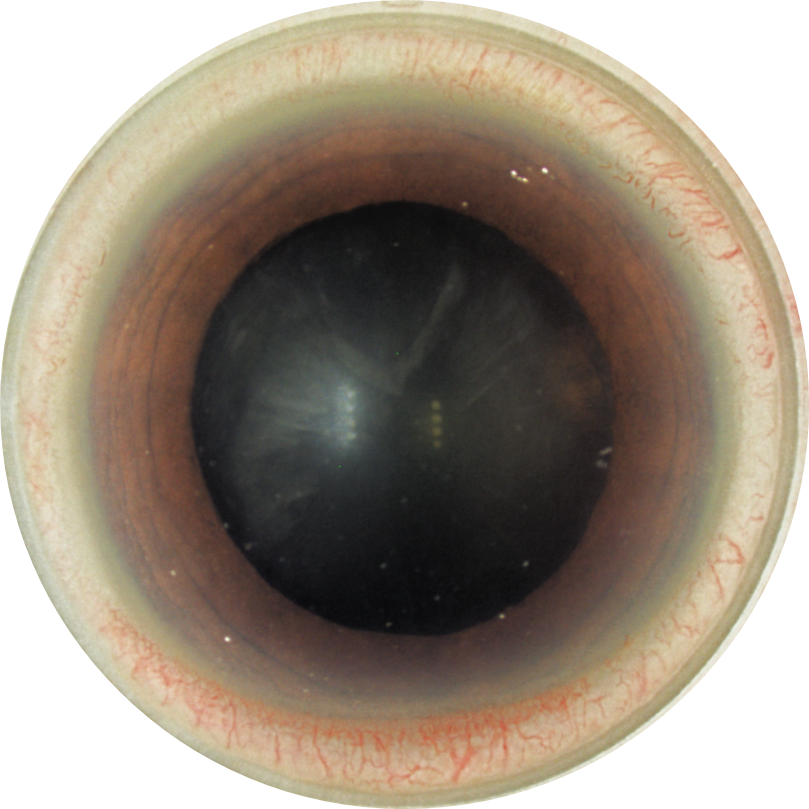
\includegraphics[width=\textwidth]{figures/eye_raw.png}}
        \only<2>{\centering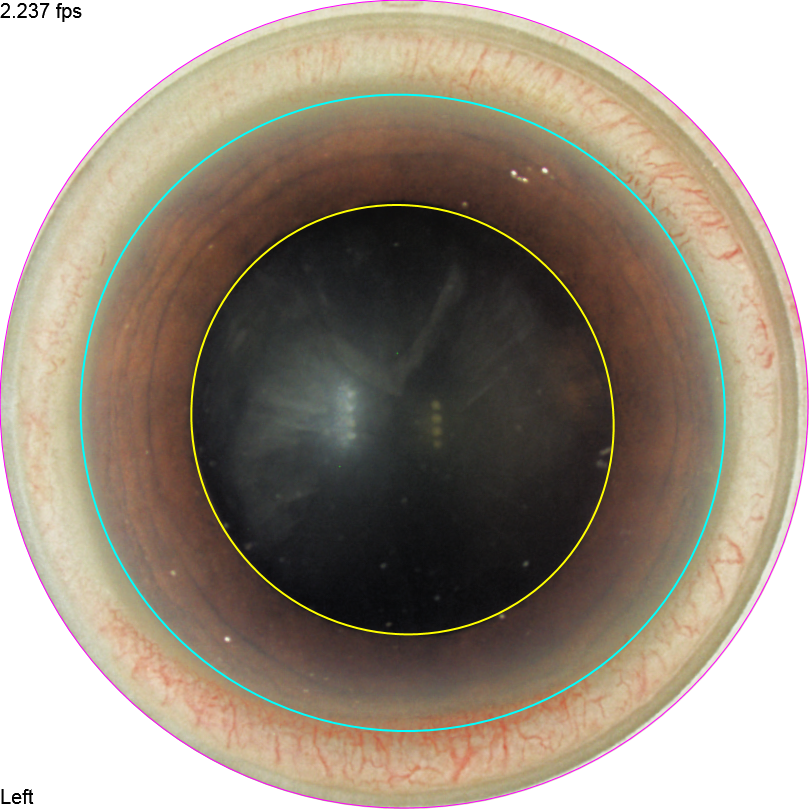
\includegraphics[width=\textwidth]{figures/eye_processed.png}}
    \end{minipage}
\end{frame}
%%%%%%%%%%%%%%%%%%%%%%%%%%%%%%%%%%%%%%%%%%%%%%%
\begin{frame}[allowframebreaks]
    \frametitle{Goals today}
        \begin{enumerate}
            \item Understand the architecture of a Deep Neural Network.
            \item Be able to diagnose most common issues in Neural Networks and to avoid them.
            \item Know the building blocks of Convolutional Neural Networks.
            \item How to use Neural Networks to measure properties hard to quantify.
            \framebreak
            \item Understand the following cartoon:
        \end{enumerate}
        \centering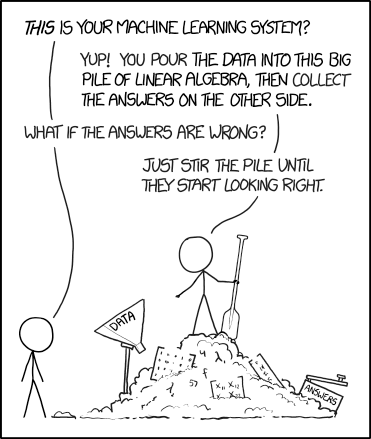
\includegraphics[height=.7\textheight]{figures/machine_learning.png}
\end{frame}
%%%%%%%%%%%%%%%%%%%%%%%%%%%%%%%%%%%%%%%%%%%%%%%
\mytoc{sec_toc}
%%%%%%%%%%%%%%%%%%%%%%%%%%%%%%%%%%%%%%%%%%%%%%%
\begin{frame}
    \frametitle{General implementation notes}
    \begin{itemize}
        \item {\bf Python} has been established as the main programming language for machine learning tasks.
        \item Libraries are provided for the implementation of well-known algorithms: {\bf SciKit Learn, Tensorflow, Keras, PyTorch} for Python, {\bf Caffe2} for C++.
        \item Python is used for a simple implementation, configuration and training, the backend uses compiled C++ code.
        \item Training is computationally expensive. Speed-up through heavily parallelized implementations, using GPUs (CUDA), and using low-rank tensor approximation.
        \item The material shown in this course is provided on
        \url{https://github.com/fablukm/}
    \end{itemize}
\end{frame}
%%%%%%%%%%%%%%%%%%%%%%%%%%%%%%%%%%%%%%%%%%%%%%%
%%%%%%%%%%%%%%%%%%%%%%%%%%%%%%%%%%%%%%%%%%%%%%%
\section{Multilayer Perceptron}
%%%%%%%%%%%%%%%%%%%%%%%%%%%%%%%%%%%%%%%%%%%%%%%
%%%%%%%%%%%%%%%%%%%%%%%%%%%%%%%%%%%%%%%%%%%%%%%
\subsection{Linear Regression as a Neural Network}
%%%%%%%%%%%%%%%%%%%%%%%%%%%%%%%%%%%%%%%%%%%%%%%
\begin{frame}[allowframebreaks]
    \frametitle{Linear Regression: Prediction}
    \begin{itemize}
        \item Consider a quantity $y\in \R^m$ which depends on $x\in\R^n$.
        \item We {\bf assume} that $y$ depends on $x$ \emph{linearly or affinely}:
        $$
        y = Wx + b\;,
        \qquad \text{for some } W\in\R^{m\times n} \text{ and } b\in \R^m
        \;.
        $$
        \item However, we do not know the exact \emph{parameters} $W$ and $b$.
        \item Need to \emph{learn} $(n+1)m$ parameters \emph{from data}.
        \item Assume we are given data points $\{(x^1, y^1), (x^2, y^2), \dots, (x^N, y^N)\}$. The data is inaccurate, subject to noise.
        \item {\bf Classical Linear Regression:} Find $W$ and $b$ subject to an optimization task, for example
        $$\min_{W\in \R^{m\times n}, b\in \R^m} \sum_{i=1}^N\left\|y^i-(Wx^i+b)\right\|_2^2$$
        {\small
        \item Two norms involved here: $l^1$ over the data, $l^2$ over the components.
        }
        \framebreak
        \item {\bf Simple constructed example:}
        \begin{tikzpicture}
  \begin{axis} [
      xlabel     = Weight (kg), % label x axis
      ylabel     = Height (cm), % label y axis
      axis lines = left, %set the position of the axes
      clip       = false,
      xmin = 40,  xmax = 105, % set the min and max values of the x-axis
      ymin = 150, ymax = 200, % set the min and max values of the y-axis
    ]
    \addplot [only marks] table {\loadedtable};
    \addplot [no markers, thick, red]
      table [y={create col/linear regression={y=y}}] {\loadedtable}
      node [anchor=west] {$\pgfmathprintnumber[precision=2, fixed zerofill]
      {\pgfplotstableregressiona} \cdot \mathrm{Weight} +
      \pgfmathprintnumber[precision=1]{\pgfplotstableregressionb}$};
  \end{axis}
\end{tikzpicture}

        \framebreak
        \item We reformulate this problem in a neural network language.
        \item There are two steps: {\bf Prediction} and {\bf Learning}.
        \item {\bf Prediciton:} Given a \emph{new} input value $x\not\in\{x^1,\dots,x^N\}$. \\
        If the parameters $W$ and $b$ are known, \emph{predict} the value $y(x)$ to be $y^\ast:=Wx+b$.
        A {\bf prediction} follows the computation graph\\[1em]
        \begin{tikzpicture}[shorten >=1pt,->,draw=black!50, node distance=\layersep]
    \tikzstyle{every pin edge}=[<-,shorten <=1pt]
    \tikzstyle{neuron}=[circle,fill=black!25,minimum size=17pt,inner sep=0pt]
    \tikzstyle{input neuron}=[neuron, fill=green!50];
    \tikzstyle{output neuron}=[neuron, fill=red!50];
    \tikzstyle{hidden neuron}=[neuron, fill=blue!50];
    \tikzstyle{annot} = [text width=4em, text centered]
    \node [input neuron] (in) at (0,0) {$x$};
    \path node [hidden neuron] (hidden) at (\layersep, 0cm) {$y^\ast:=Wx+b$};
    \node[output neuron, right of=hidden] (out) {$y:=y^\ast$};
    \path (in) edge (hidden);
    \path (hidden) edge (out);
    \node[annot, above of=in, node distance=4.5em] (t_in) {Input};
    \node[annot, above of=hidden, node distance=5em] (t_hidden) {Hidden layer};
    \node[annot, above of=out, node distance=5em] (t_out) {Output};
\end{tikzpicture}

        \item For further purposes, we put the linear combination into a \emph{hidden layer} and define the output to be the output of the hidden layer.
        \framebreak
        \item The same graph, but component-by-component:
        \begin{tikzpicture}[shorten >=1pt,->,draw=black!50, node distance=\layersep, scale=.7]
    \tikzstyle{every pin edge}=[<-,shorten <=1pt]
    \tikzstyle{neuron}=[circle,fill=black!25,minimum size=10pt,inner sep=0pt]
    \tikzstyle{input neuron}=[neuron, fill=green!50];
    \tikzstyle{output neuron}=[neuron, fill=red!50];
    \tikzstyle{hidden neuron}=[neuron, fill=blue!50];
    \tikzstyle{annot} = [text width=4em, text centered]

    \node [input neuron] (in-1) at (0,0) {$x_1$};
    \node [input neuron] (in-2) at (0,-1) {$x_2$};
    \node [input neuron] (in-3) at (0,-2) {$\vdots$};
    \node [input neuron] (in-4) at (0,-3) {$x_n$};

    \path node [hidden neuron] (hidden-1) at (\layersep, 0cm) {$y^\ast_1$};
    \path node [hidden neuron] (hidden-2) at (\layersep, -1) {$y^\ast_2$};
    \path node [hidden neuron] (hidden-3) at (\layersep, -2) {$\vdots$};
    \path node [hidden neuron] (hidden-4) at (\layersep, -3) {$y^\ast_m$};
    \node[output neuron, right of=hidden-1] (out-1) {$y_1$};
    \node[output neuron, right of=hidden-2] (out-2) {$y_2$};
    \node[output neuron, right of=hidden-3] (out-3) {$\vdots$};
    \node[output neuron, right of=hidden-4] (out-4) {$y_m$};

    \foreach \source in {1,...,4}
        \foreach \dest in {1,...,4}
            \path (in-\source) edge (hidden-\dest);

    \foreach \source in {1,...,4}
        \path (hidden-\source) edge (out-\source);

    \node[annot, above of=in-1, node distance=2em] (t_in) {Input};
    \node[annot, above of=hidden-1, node distance=2em] (t_hidden) {Hidden};
    \node[annot, above of=out-1, node distance=2em] (t_out) {Output};
\end{tikzpicture}


        where
        {\small
        \begin{equation*}
            \begin{split}
                y^\ast_k &:= \sum_{j=1}^n w_{kj}x_j + b_k
                \;, \qquad k=1,\dots, m
                \;,\\
                y_k & := y^\ast_k
                \;, \qquad k=1,\dots, m
                \;,
            \end{split}
        \end{equation*}
        $w_{kj}$ and $b$ are \emph{weights which are determined iteratively to fit the data.}}
    \end{itemize}
\end{frame}
%%%%%%%%%%%%%%%%%%%%%%%%%%%%%%%%%%%%%%%%%%%
\begin{frame}
    \frametitle{Linear Regression: Training}
    \begin{itemize}
        \item {\bf Loss function: } To \emph{learn} the weights $w_{kj}$, we minimize the {\bf mean squared error}. For one sample $(x^i, y^i)$, it is defined as
        $$
        \mse(x^i, y^i):=\frac{1}{m}\sum_{k=1}^m \left(y^i_k - \left(Wx^i+b\right)_k\right)^2
        \;.
        $$
        \item {\bf Gradient descent:} Find weights $W, b$ such that $\mse$ is minimal. Standard iteration:
        \begin{equation*}
            \begin{split}
                w_{kj; \text{new}} &:= w_{kj; \text{current}} - \learningrate \frac{\partial \mse}{\partial w_{kj}}
                \;,\\
                b_{k; \text{new}} &:= b_{k; \text{current}} - \learningrate \frac{\partial \mse}{\partial b_k}
                \;,
            \end{split}
        \end{equation*}
        with \emph{randomly initialized weights} $w_{kj; \text{start}}$ and $b_{j; \text{start}}$,\\
        with \emph{learning rate} $\learningrate>0$.
        \item Linear regression with loss $\mse$: Derivatives easy to compute.
    \end{itemize}
\end{frame}
%%%%%%%%%%%%%%%%%%%%%%%%%%%%%%%%%%%%%%%%%%%
\begin{frame}
    \frametitle{Intuition for Gradient Descent}
    \centering
    \only<1>{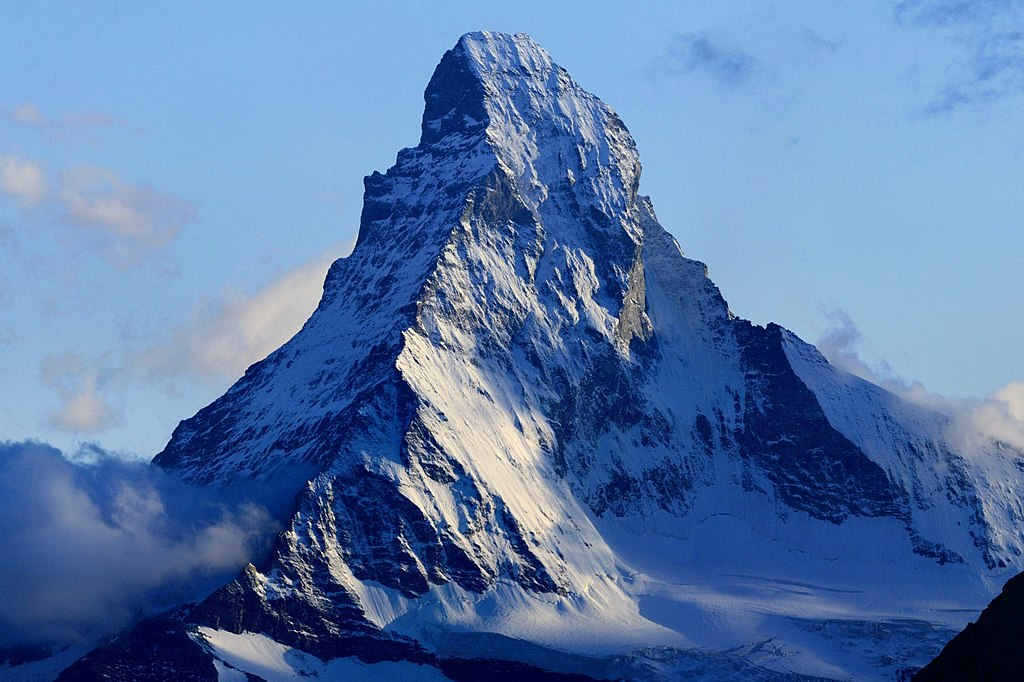
\includegraphics[width=.7\textwidth]{figures/mountain.jpg}}
    \only<2>{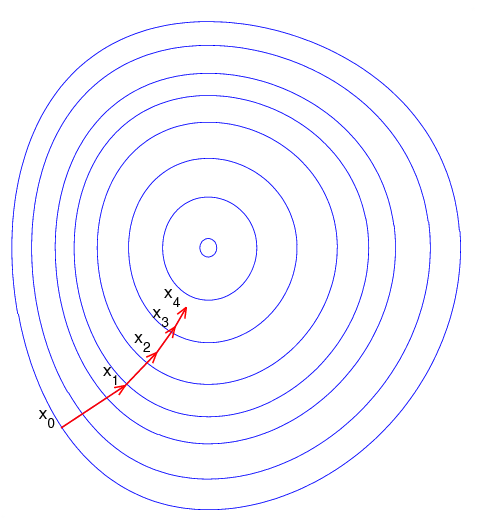
\includegraphics[width=.6\textwidth]{figures/gradientdescent1.png}}
    \only<3>{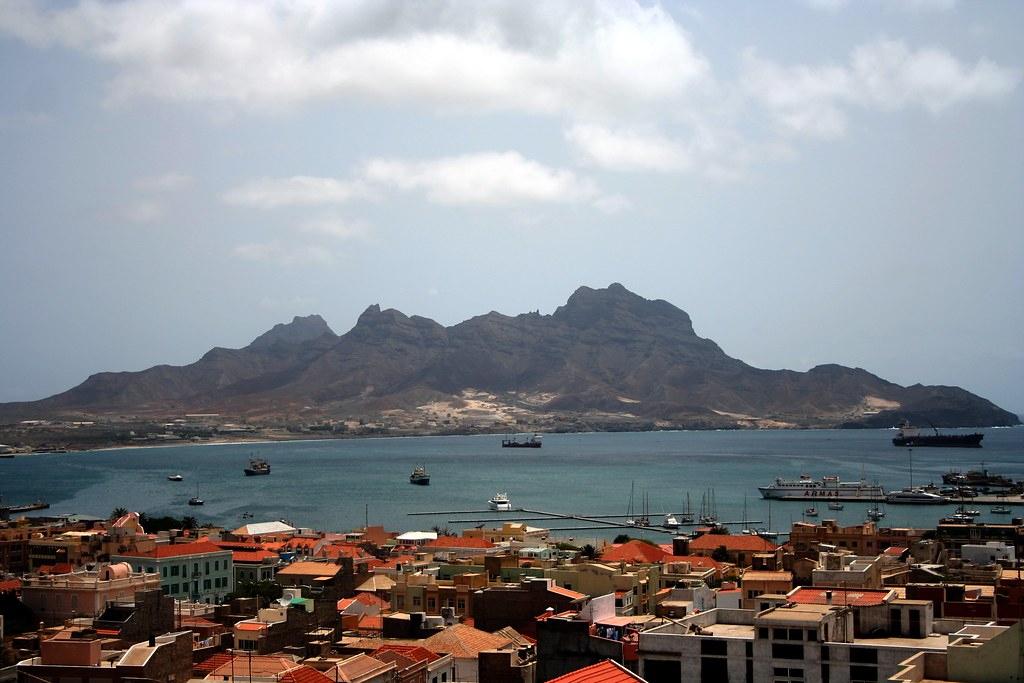
\includegraphics[width=.7\textwidth]{figures/mountain2.jpg}}
    \only<4>{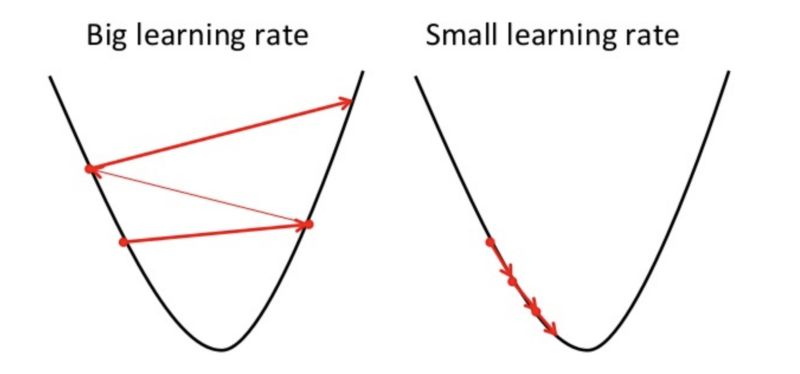
\includegraphics[width=\textwidth]{figures/gradientdescent2.png}}
    \only<5>{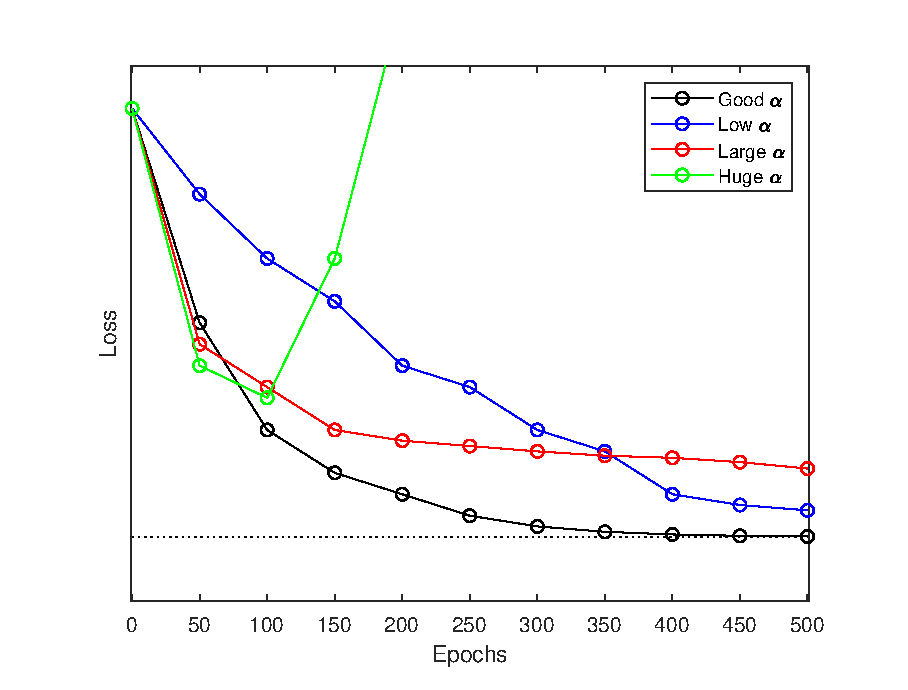
\includegraphics[width=.9\textwidth]{figures/gradientdescent3.eps}}
\end{frame}
%%%%%%%%%%%%%%%%%%%%%%%%%%%%%%%%%%%%%%%%%%%
\begin{frame}
    \frametitle{Remarks about Gradient Descent}
        \begin{enumerate}
            \item The performance of the algorithm depends on the choice of a learning rate $\learningrate>0$.
            \begin{itemize}
                \item Large learning rate: Fast descent at first, may not converge.
                \item Small learning rate: Slow convergence overall.
            \end{itemize}
            \item No guarantee to find global minimum for a arbitrary loss functions.
            \item {\bf In practise:} Better minimization schemes, derived from gradient descent: ADAM, Stochastic GD.
            \item {\bf In practise:} A tolerance and a maximal number of iterations should be chosen as well.
            \item {\bf Definition:} (Only) here, we call one iteration one \emph{epoch}.
        \end{enumerate}
    \centering $\boldsymbol{\Rightarrow}$ {\bf Parameters} are learned by minimization of the loss function, but {\bf hyperparameters} are determining the algorithm, and are chosen at the beginning!
\end{frame}
%%%%%%%%%%%%%%%%%%%%%%%%%%%%%%%%%%%%%%%%%%%
\begin{frame}
    \frametitle{Towards Neural Networks 1: Hidden Layers}
    \begin{minipage}{.5\textwidth}
        \begin{tikzpicture}[shorten >=1pt,->,draw=black!50, node distance=\layersep, scale=.7]
    \tikzstyle{every pin edge}=[<-,shorten <=1pt]
    \tikzstyle{neuron}=[circle,fill=black!25,minimum size=17pt,inner sep=0pt]
    \tikzstyle{input neuron}=[neuron, fill=green!50];
    \tikzstyle{output neuron}=[neuron, fill=red!50];
    \tikzstyle{hidden neuron}=[neuron, fill=blue!50];
    \tikzstyle{annot} = [text width=4em, text centered]

    \node [input neuron] (in-1) at (0,0) {$x_1$};
    \node [input neuron] (in-2) at (0,-1) {$x_2$};
    \node [input neuron] (in-3) at (0,-2) {$\vdots$};
    \node [input neuron] (in-4) at (0,-3) {$x_n$};

    \path node [hidden neuron] (hidden-1) at (\layersep, 0cm) {$y^\ast_1$};
    \path node [hidden neuron] (hidden-2) at (\layersep, -1) {$\vdots$};
    \path node [hidden neuron] (hidden-3) at (\layersep, -2) {$y^\ast_{m_1}$};
    \node[output neuron, right of=hidden-1] (out-1) {$y_1$};
    \node[output neuron, right of=hidden-2] (out-2) {$y_2$};
    \node[output neuron, right of=hidden-3] (out-3) {$\vdots$};
    \node[output neuron, right of=hidden-4] (out-4) {$y_m$};

    \foreach \source in {1,...,4}
        \foreach \dest in {1,...,3}
            \path (in-\source) edge (hidden-\dest);

    \foreach \source in {1,...,3}
        \foreach \dest in {1,...,4}
        \path (hidden-\source) edge (out-\dest);

    \node[annot, above of=in-1, node distance=2em] (t_in) {Input};
    \node[annot, above of=hidden-1, node distance=2em] (t_hidden) {Hidden};
    \node[annot, above of=out-1, node distance=2em] (t_out) {Output};
\end{tikzpicture}

    \end{minipage}
    \begin{minipage}{.4\textwidth}
        \begin{itemize}
            \item Change the size of the hidden layer to $m_1\neq m$.
            \item Compute $y_k$ by another linear combination of the $y_l^{\ast}$.
            \item More weights to learn: $W^{[\text{in},\text{hidden}]}\in\R^{m_1\times n}$ and $W^{[\text{hidden}, \text{out}]}\in\R^{m\times m}$.
            \item Gradient descent needs derivatives w.r.~to both weights.
            \item[$\boldsymbol{?}$] {\bf What will be different now?}
        \end{itemize}
    \end{minipage}
\end{frame}
%%%%%%%%%%%%%%%%%%%%%%%%%%%%%%%%%%%%%%%%%%%
\begin{frame}
    \frametitle{Towards Neural Networks 2: Hidden Layers}
    \begin{itemize}
        \item Linear of linear is linear: {\bf Nothing changed.}
        \item Add one more hidden layer with $m_2$ nodes.
        \item Hidden layer 1 \emph{gets propagated} by linear combination to Hidden layer 2.
        \item Introduces weights $W^{[1,2]}\in \R^{m_2\times m_1}$.
        \item[$\boldsymbol{?}$] {\bf What will be different now?}
    \end{itemize}

    \centering \begin{tikzpicture}[shorten >=1pt,->,draw=black!50, node distance=\layersep, scale=.7]
    \tikzstyle{every pin edge}=[<-,shorten <=1pt]
    \tikzstyle{neuron}=[circle,fill=black!25,minimum size=17pt,inner sep=0pt]
    \tikzstyle{input neuron}=[neuron, fill=green!50];
    \tikzstyle{output neuron}=[neuron, fill=red!50];
    \tikzstyle{hidden neuron}=[neuron, fill=blue!50];
    \tikzstyle{annot} = [text width=4em, text centered]

    \node [input neuron] (in-1) at (0,0) {$x_1$};
    \node [input neuron] (in-2) at (0,-1.1) {$x_2$};
    \node [input neuron] (in-3) at (0,-2.2) {$\vdots$};
    \node [input neuron] (in-4) at (0,-3.3) {$x_n$};

    \path node [hidden neuron] (hidden1-1) at (\layersep, 0cm) {$h^{[1]}_1$};
    \path node [hidden neuron] (hidden1-2) at (\layersep, -1.1cm) {$\vdots$};
    \path node [hidden neuron] (hidden1-3) at (\layersep, -2.3cm) {$h^{[1]}_{m_1}$};
    \path node [hidden neuron, right of=hidden1-1] (hidden2-1) {$h^{[2]}_1$};
    \path node [hidden neuron, right of=hidden1-2] (hidden2-2) {$\vdots$};
    \path node [hidden neuron, right of=hidden1-3] (hidden2-3) {$h^{[2]}_{m_2}$};
    \node[output neuron, right of=hidden2-1] (out-1) {$y_1$};
    \node[output neuron, right of=hidden2-2] (out-2) {$y_2$};
    \node[output neuron, right of=hidden2-3] (out-3) {$y_m$};

    \foreach \source in {1,...,4}
        \foreach \dest in {1,...,3}
            \path (in-\source) edge (hidden1-\dest);

    \foreach \source in {1,...,3}
        \foreach \dest in {1,...,3}
            \path (hidden1-\source) edge (hidden2-\dest);

    \foreach \source in {1,...,3}
        \foreach \dest in {1,...,3}
        \path (hidden2-\source) edge (out-\dest);

    \node[annot, above of=in-1, node distance=2em] (t_in) {Input};
    \node[annot, above of=hidden1-1, node distance=2em] (t_hidden) {HL 1};
    \node[annot, above of=hidden2-1, node distance=2em] (t_ac) {HL 2};
    \node[annot, above of=out-1, node distance=2em] (t_out) {Output};
\end{tikzpicture}

\end{frame}
%%%%%%%%%%%%%%%%%%%%%%%%%%%%%%%%%%%%%%%%%%%
\begin{frame}
    \frametitle{Towards Neural Networks 3: Activation functions}
    \begin{itemize}
        \item {\bf Still nothing has changed.}
        \item {\bf Idea:} Apply a non-linear {\bf Activation Function} $g$ to the output of a hidden layer.
        \item Several activation functions have been proposed for different purposes.
        \item Replace a hidden node $h^{[l]}_{k}$ (the $k$-th node in the $l$-th layer) by
        $$
            h^{[l]}_k := g(h^{[l]}_k)
        $$
    \end{itemize}
    %
    \centering\begin{tikzpicture}[shorten >=1pt,->,draw=black!50, node distance=3cm, scale=.7]
    \tikzstyle{every pin edge}=[<-,shorten <=1pt]
    \tikzstyle{neuron}=[circle,fill=black!25,minimum size=17pt,inner sep=0pt]
    \tikzstyle{hidden neuron}=[neuron, fill=blue!50];
    \tikzstyle{annot} = [text width=5em, text centered]

    \path node [hidden neuron] (hidden1) at (\layersep, 0cm) {$\hat{h}^{[l]}_k$};
    \path node [hidden neuron, right of=hidden1] (hidden2) {$h^{[l]}_k:= g(\hat{h}^{[l]}_k)$};



    \path (hidden1) edge (hidden2);


    \node[annot, above of=hidden1, node distance=4em] (t_hidden) {Linear comb.};
    \node[annot, above of=hidden2, node distance=4em] (t_ac) {Activation};
\end{tikzpicture}

\end{frame}
%%%%%%%%%%%%%%%%%%%%%%%%%%%%%%%%%%%%%%%%%%%
\subsection{Multilayer Perceptron: Definition}
%%%%%%%%%%%%%%%%%%%%%%%%%%%%%%%%%%%%%%%%%%%
%%%%%%%%%%%%%%%%%%%%%%%%%%%%%%%%%%%%%%%%%%%
\begin{frame}[allowframebreaks]
    \frametitle{Multilayer Perceptron: Forward}
        \centering\begin{tikzpicture}[shorten >=1pt,->,draw=black!50, node distance=\layersep]
    \tikzstyle{every pin edge}=[<-,shorten <=1pt]
    \tikzstyle{neuron}=[circle,fill=black!25,minimum size=17pt,inner sep=0pt]
    \tikzstyle{input neuron}=[neuron, fill=green!50];
    \tikzstyle{output neuron}=[neuron, fill=red!50];
    \tikzstyle{hidden neuron}=[neuron, fill=blue!50];
    \tikzstyle{annot} = [text width=4em, text centered]

    % Draw the input layer nodes
    \foreach \name / \y in {1,...,4}
    % This is the same as writing \foreach \name / \y in {1/1,2/2,3/3,4/4}
        \node[input neuron] (I-\name) at (0,-\y) {$x_{\y}$};

    % Draw the hidden layer nodes
    \foreach \name / \y in {1,...,5}
        \path[yshift=0.5cm]
            node[hidden neuron] (H1-\name) at (\layersep,-\y cm) {$h^{[1]}_{\y}$};

    % Draw the hidden layer nodes
    \foreach \name / \y in {1,...,5}
        \path[yshift=0.5cm]
            node[hidden neuron, right of=H1-\name] (Hdots-\name) at (\layersep,-\y cm) {$\dots$};


    % Draw the hidden layer nodes
    \foreach \name / \y in {1,...,4}
        \path[yshift=0.5cm]
            node[hidden neuron, right of=Hdots-\name] (H2-\name) {$h^{[L]}_{\y}$};

    % Draw the output layer node
    \node[output neuron, right of=H2-3] (O) {$y$};

    % Connect every node in the input layer with every node in the
    % hidden layer.
    \foreach \source in {1,...,4}
        \foreach \dest in {1,...,5}
            \path (I-\source) edge (H1-\dest);

    \foreach \source in {1,...,5}
        \foreach \dest in {1,...,5}
            \path (H1-\source) edge (Hdots-\dest);

    % Connect every node in the first hidden layer with every node in the
    % hidden layer 2.
    \foreach \source in {1,...,5}
        \foreach \dest in {1,...,4}
            \path (Hdots-\source) edge (H2-\dest);

    % Connect every node in the hidden layer with the output layer
    \foreach \source in {1,...,4}
        \path (H2-\source) edge (O);

    % Annotate the layers
    \node[annot,above of=H1-1, node distance=1cm] (hl1) {Hidden layer};
    \node[annot,above of=H2-1, node distance=1cm] (hl2) {Hidden layer};
    \node[annot,left of=hl1,] {Input layer};
    \node[annot,right of=hl2,] {Output layer};
\end{tikzpicture}

        \framebreak
        %
        \begin{definition}[Multilayer Perceptron (MLP)]
            A multilayer perceptron (\emph{neural network}) architecture is defined by
            \begin{enumerate}
                \item the input size $m_0$
                \item the number of hidden layers $L$
                \item the size of each hidden layers $\{m_l\}_{l=1,\dots,L}$
                \item the activation function applied to hidden layer $l$ $\{g^{[l]}\}_{l=1,\dots,L}$
                \item the output size $m_{L+1}$
            \end{enumerate}
            To run an input through the MLP, one needs for each layer
            \begin{equation*}
                \begin{split}
                    \text{weights }& W^{[l, l+1]}\in \R^{m_{l+1}\times m_l}
                    \;,\qquad l\in\{0, \dots, L\}
                    \;,\\
                    \text{ biases }& b^{[l, l+1]} \in \R^{m_{l+1}}
                    \;,\qquad\qquad l\in\{0, \dots, L\}
                    \;.
                \end{split}
            \end{equation*}
        \end{definition}
    \framebreak
    \begin{itemize}
        \item Forward step (if the weights are known):
        \begin{enumerate}
            \item We start with an input $x=(x_1,\dots,x_{m_0})\in \R^{m_0}$.
            \item Compute a linear combination of the input to obtain the nodes in the first hidden layer, and apply an activation function $g^{[1]}$: $$h^{[1]}:=g^{[1]}\left(W^{[0,1]}x+b^{[0,1]}\right)\;.$$
            \item For $l=1,\dots,L-1$, use layer $l$ as input for layer $l+1$:
            $$h^{[l+1]}:=g^{[l]}\left(W^{[l,l+1]}h^{[l]}+b^{[l+1]}\right)\;.$$
            \item Compute the output:
            $$y:=g^{[L]}\left(W^{[L,L+1]}h^{[L]}+b^{[L+1]}\right)\;.$$
        \end{enumerate}
        \item A MLP with input $x$ is a composition of maps. \\
        {\bf Notation:} $y=\nn(x)$.
    \end{itemize}
\end{frame}
%%%%%%%%%%%%%%%%%%%%%%%%%%%%%%%%%%%%%%%%%%%
%%%%%%%%%%%%%%%%%%%%%%%%%%%%%%%%%%%%%%%%%%%
\subsection{Activation Functions}
%%%%%%%%%%%%%%%%%%%%%%%%%%%%%%%%%%%%%%%%%%%
\begin{frame}[allowframebreaks]
    \frametitle{Activation Functions}
    \centering{\large{\bf The $\tanh$ activation function}}

    \begin{itemize}
        \item Consider $g(\eta):=\tanh(\eta):= \frac{e^{\eta}-e^{-\eta}}{e^{\eta}+e^{-\eta}}$.
        \item Derivative: $g'(\eta) = 1-\left(g(\eta)\right)^2 $
        \item $\displaystyle\lim_{\eta\to-\infty} g(\eta) = -1$, $\displaystyle\lim_{\eta\to\infty} g(\eta) = 1$
        \item Used for \emph{Binary Classification}: ``Is it a car or a house?''
    \end{itemize}
    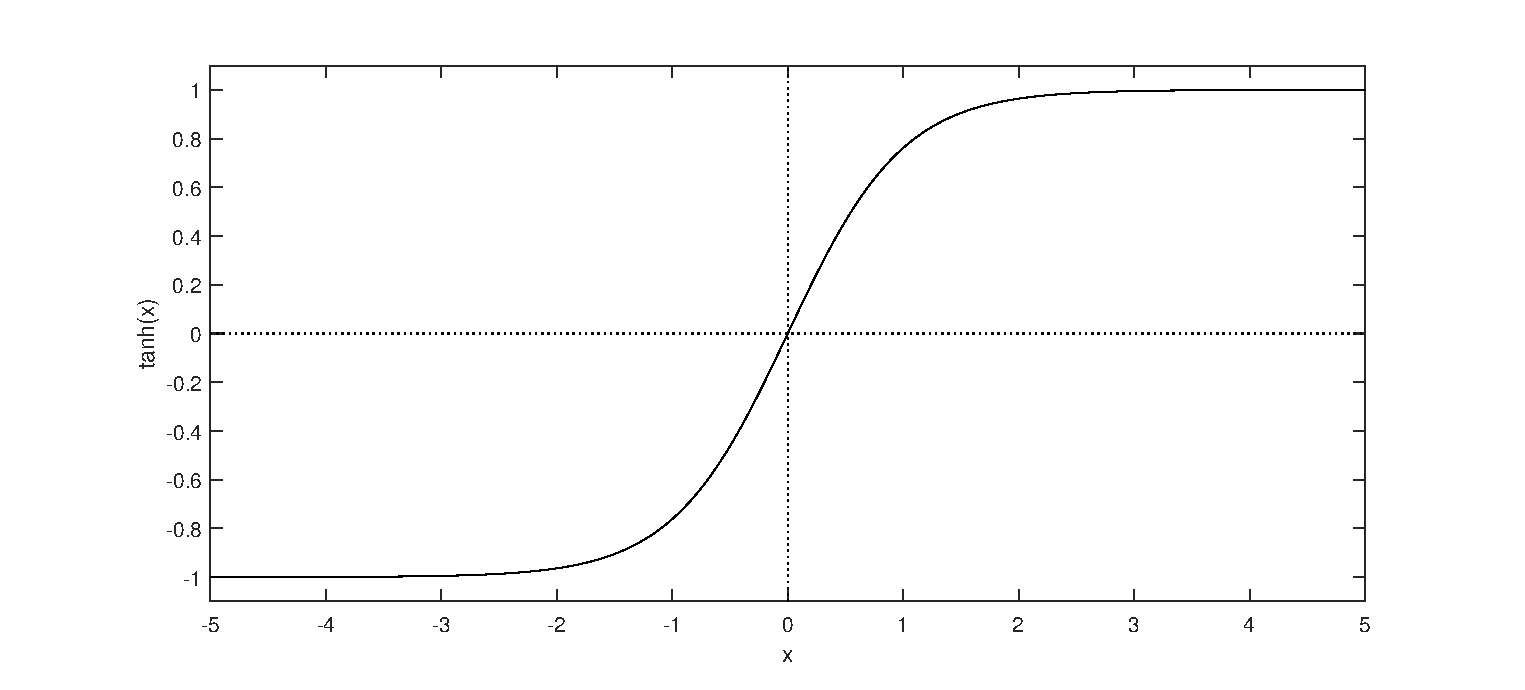
\includegraphics[width=.7\textwidth]{figures/tanh.eps}
    \framebreak

    {\large{\bf The $\relu$ activation function}}

    \begin{itemize}
        \item Consider $g(\eta):=\relu(\eta):= \max\{0, \eta\}$.
        \item Derivative piecewise: $g'(\eta) = \indicator_{(0, \infty]}(\eta)$ for $\eta\neq 0$.
        \item Drops negative values: ``Activates only positive neurons''.
    \end{itemize}
    \centering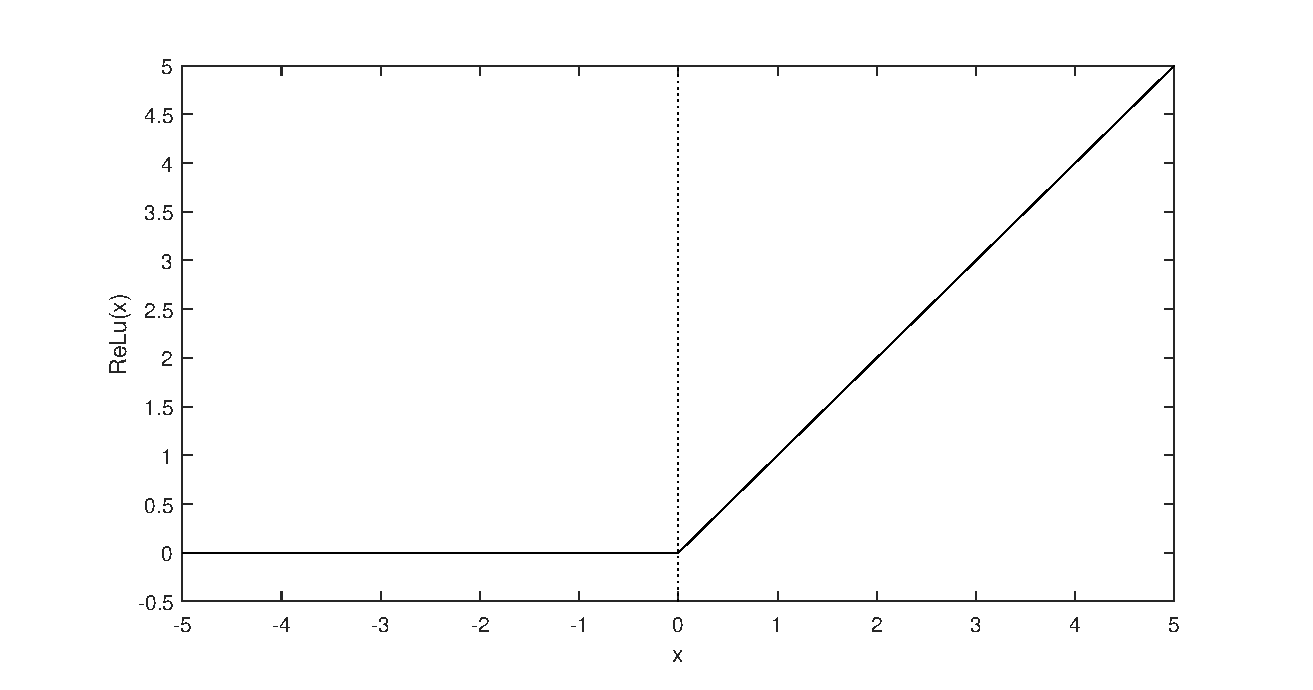
\includegraphics[width=.7\textwidth]{figures/relu.eps}
    \framebreak

    {\large{\bf The logistic activation function $\sigma$}}

    \begin{itemize}
        \item Consider $g(\eta):=\sigma(\eta):= \frac{1}{1+e^{-\eta}}$.
        \item Derivative piecewise: $g'(\eta) = g(\eta)(1-g(\eta))$.
        \item Binary $0-1$ classification.
    \end{itemize}
    \centering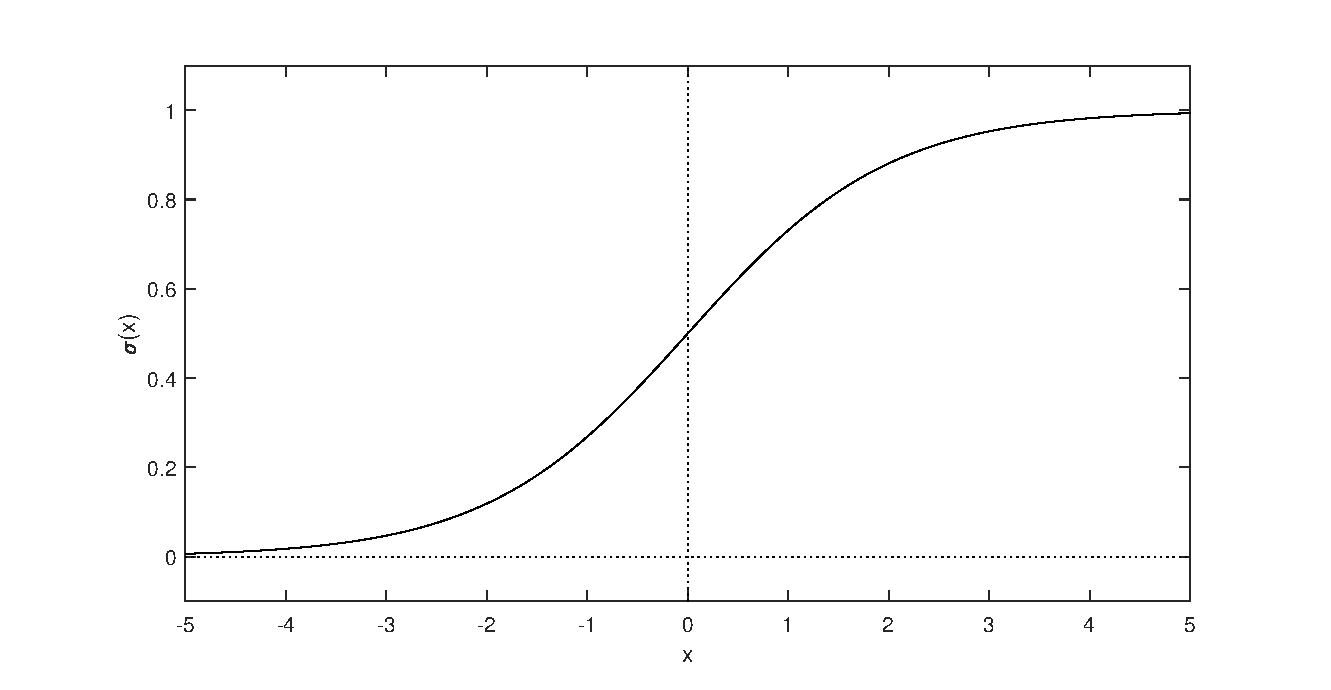
\includegraphics[width=.7\textwidth]{figures/sigmoid.eps}
    \framebreak

    {\large{\bf The Softmax activation function}}

    \begin{itemize}
        \item Consider $g: \R^m\to \R^m$ written as $(g_1, \dots, g_m)$. Define
        $$
            g_k(\eta_1, \dots, \eta_m) := \frac{e^{\eta_k}}{\sum_je^{\eta_j}}
            \;,\quad k=1,\dots,m
            \;,
        $$
        \item Examples:
            \begin{equation*}
                \begin{split}
                    g(0,1,0)&\simeq(0.2, 0.6, 0.2)\\
                    g(0,10,0)&\simeq(0, 1, 0)\\
                    g(0,-10,0)&\simeq(0.5, 0, 0.5)
                \end{split}
            \end{equation*}
        \item ``Scales to $[0,1]$ and discriminates small values.''
        \item $\sum_k g_k=1$: Can be interpreted as a discrete probability over $\eta$.
        \item ``Is it a dog, a cat, a bird, a house, or a car?''
        \item Derivative piecewise: $\frac{\partial g_k}{\partial \eta_j} = g_k(\delta_{kj}-g_j)$ .
    \end{itemize}
\end{frame}
%%%%%%%%%%%%%%%%%%%%%%%%%%%%%%%%%%%%%%%%%%%
\begin{frame}
    \frametitle{Lab: MLP for digit recognition 1}
    \begin{minipage}{.7\textwidth}
        {\small
        \begin{itemize}
            \item {\bf Classification Task:} Given an image of a handwritten digit, detect the digit on the image.
            \item {\bf Input:} Greyscale image $28\times 28$: $m_0=28^2=784$.
            \item {\bf Output:} $\mathbf{p}=(p_0, \dots, p_9)\in [0,1]^{10}$. $p_k$: probability that $k$ on the image.
            \item Choice of last activation function $g^{[L]}$?
            \item {\bf Architecture:} We choose a MLP with $L=2, m_1=m_2=512$. Clearly, $m_3=10$.
            \item {\bf Activation function:} $g^{[1]}=\relu$.
        \end{itemize}
        }
    \end{minipage}
    \begin{minipage}{.25\textwidth}
        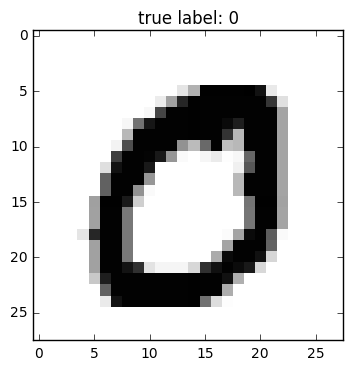
\includegraphics[width=\textwidth]{figures/mnist_data.png}
    \end{minipage}
\end{frame}
%%%%%%%%%%%%%%%%%%%%%%%%%%%%%%%%%%%%%%%%%%%
\begin{frame}
    \frametitle{Loss function for classification}
        {\small
        \begin{itemize}
            \item {\bf Softmax:} Output is a discrete probability distribution.
            \item {\bf Dataset:} $\dataset=\{(x^i, y^i)\}_{i=1,\dots,N}$ with correct labels $y^i_k\in\{0,1\}$
            \item True outputs are either $0$ or $1$ for each digit.
            \item {\bf Cross-entropy loss for one sample:} (set $0\log(0):=0$)
                \begin{equation*}
                    \begin{split}
                        \loss(y_{\text{pred}}, y_{\text{true}}) &=
                            -\sum_{k=0}^9 \log(y_{\text{pred}})y_{\text{true}} \\
                            &\stackrel{\text{binary}}{=}
                            -\sum_{k=0}^9 y_{\text{true}}\log(y_{\text{pred}})
                                + (1-y_{\text{true}}) \log(1-y_{\text{pred}})
                            \;.
                    \end{split}
                \end{equation*}
            \item If true label is $1$ and predicted tends to $0$: $\loss$ explodes.
            \item Avoid numerical instabilities in implementation.
            \item Loss for entire dataset:
            $$
            \loss_{\text{ce}}(\nn; \dataset) :=
                -\frac{1}{N}\sum_{i=1}^N \loss(\nn(x^i), y^i)
                \;.
            $$

        \end{itemize}
        }
\end{frame}
%%%%%%%%%%%%%%%%%%%%%%%%%%%%%%%%%%%%%%%%%%%
\subsection{Backpropagation}
%%%%%%%%%%%%%%%%%%%%%%%%%%%%%%%%%%%%%%%%%%%
%%%%%%%%%%%%%%%%%%%%%%%%%%%%%%%%%%%%%%%%%%%
\begin{frame}[allowframebreaks]
    \frametitle{Multilayer Perceptron: Learning}
    \begin{itemize}
        \item {\bf Ground truth:} Given a labeled dataset $\dataset=\{(x^i, y^i)\}_{i=1,\dots,N}$.
        \item We call $x^i$ \emph{features} and $y^i$ \emph{labels}.
        \item For theoretical purposes: All parameters in one vector $\boldsymbol{\xi}$, loss dependent on $\boldsymbol{\xi}$.
        \item Need to minimize a {\bf loss function} (``error'') $\loss(\boldsymbol{\xi}; \dataset)$:
        $$
        \boldsymbol{\xi}^\ast = \arg\min_{\boldsymbol{\xi}} \loss(\boldsymbol{\xi}; \dataset)
        \;.
        $$
        \item {\bf Gradient descent} with learning rate $\learningrate>0$:
        $$
            \boldsymbol{\xi}^{\text{new}} := \boldsymbol{\xi}^{\text{current}}
            - \learningrate \nabla_{\boldsymbol{\xi}}J(\boldsymbol{\xi}^{\text{current}};\dataset)
        $$
    \end{itemize}
    \framebreak
    \centering\begin{tikzpicture}[shorten >=1pt,->,draw=black!50, node distance=\layersep]
    \tikzstyle{every pin edge}=[<-,shorten <=1pt]
    \tikzstyle{neuron}=[circle,fill=black!25,minimum size=17pt,inner sep=0pt]
    \tikzstyle{input neuron}=[neuron, fill=green!50];
    \tikzstyle{output neuron}=[neuron, fill=red!50];
    \tikzstyle{hidden neuron}=[neuron, fill=blue!50];
    \tikzstyle{annot} = [text width=4em, text centered]

    % Draw the input layer nodes
    \foreach \name / \y in {1,...,4}
    % This is the same as writing \foreach \name / \y in {1/1,2/2,3/3,4/4}
        \node[input neuron] (I-\name) at (0,-\y) {$x_{\y}$};

    % Draw the hidden layer nodes
    \foreach \name / \y in {1,...,5}
        \path[yshift=0.5cm]
            node[hidden neuron] (H1-\name) at (\layersep,-\y cm) {$h^{[1]}_{\y}$};

    % Draw the hidden layer nodes
    \foreach \name / \y in {1,...,5}
        \path[yshift=0.5cm]
            node[hidden neuron, right of=H1-\name] (Hdots-\name) at (\layersep,-\y cm) {$\dots$};


    % Draw the hidden layer nodes
    \foreach \name / \y in {1,...,4}
        \path[yshift=0.5cm]
            node[hidden neuron, right of=Hdots-\name] (H2-\name) {$h^{[L]}_{\y}$};

    % Draw the output layer node
    \node[output neuron, right of=H2-3] (O) {$y$};

    % Connect every node in the input layer with every node in the
    % hidden layer.
    \foreach \source in {1,...,4}
        \foreach \dest in {1,...,5}
            \path (I-\source) edge (H1-\dest);

    \foreach \source in {1,...,5}
        \foreach \dest in {1,...,5}
            \path (H1-\source) edge (Hdots-\dest);

    % Connect every node in the first hidden layer with every node in the
    % hidden layer 2.
    \foreach \source in {1,...,5}
        \foreach \dest in {1,...,4}
            \path (Hdots-\source) edge (H2-\dest);

    % Connect every node in the hidden layer with the output layer
    \foreach \source in {1,...,4}
        \path (H2-\source) edge (O);

    % Annotate the layers
    \node[annot,above of=H1-1, node distance=1cm] (hl1) {Hidden layer};
    \node[annot,above of=H2-1, node distance=1cm] (hl2) {Hidden layer};
    \node[annot,left of=hl1,] {Input layer};
    \node[annot,right of=hl2,] {Output layer};
\end{tikzpicture}

    \framebreak
    \begin{minipage}{.6\textwidth}
        {\small
        \begin{itemize}
            \item $L=1$, $m_1=m_{2}=1$.
            \item No indices, and $W\in\R^{m_0}$ vector.
            \item {\color{red}Red:} computable. \\
            {\color{blue}Blue:} already computed.
            \item Chain rule:
            \begin{enumerate}
                \item First step (analogous for bias):
                $$
                \frac{\partial\loss}{\partial \hat{h}} =
                {\color{red}
                \frac{\partial\loss}{\partial y} \frac{\partial y}{\partial \hat{h}}}
                =
                {\color{red}\frac{\partial\loss}{\partial y}} {\color{red}g'}
                \;.
                $$
                \item Second step:
                $$
                \frac{\partial\loss}{\partial W_k} =
                {\color{blue}\frac{\partial\loss}{\partial \hat{h}}}
                {\color{red}
                \frac{\partial \hat{h}}{\partial W_k}
                }=
                {\color{blue}\frac{\partial\loss}{\partial \hat{h}}}
                {\color{red}
                x_k
                }
                \;.
                $$
                (analogous for $\frac{\partial}{\partial b}$).
            \end{enumerate}
        \end{itemize}
        }
    \end{minipage}
    \begin{minipage}{.3\textwidth}
        \begin{tikzpicture}[shorten >=1pt,->,draw=black!50, node distance=\layersep]
    \tikzstyle{every pin edge}=[<-,shorten <=1pt]
    \tikzstyle{neuron}=[rectangle,fill=black!25,minimum size=17pt,inner sep=0pt]
    \tikzstyle{input neuron}=[neuron, fill=green!50];
    \tikzstyle{output neuron}=[neuron, fill=red!50];
    \tikzstyle{hidden neuron}=[neuron, fill=blue!50];
    \tikzstyle{loss neuron}=[neuron, fill=yellow!50];
    \tikzstyle{annot} = [text width=4em, text centered]

    \node [input neuron] (in) at (0,0) {$x$};
    \path node [hidden neuron, below = .5cm of in] (hidden1) {$\hat{h}=Wx+b$};
    \path node [output neuron, below = .5cm of hidden1] (hidden1act) {$y:=g(\hat{h})$};
    \node[loss neuron, below = .5cm of hidden1act] (loss) {$\loss(W, b; x, y)$};
    \path (in) edge (hidden1);
    \path (hidden1) edge (hidden1act);
    \path (hidden1act) edge (loss);
\end{tikzpicture}

    \end{minipage}
    \framebreak
    \begin{itemize}
        \item Gradient descent:
        \begin{equation*}
            \begin{split}
                W_k^{\text{new}} &=
                W_k^{\text{current}} -
                \learningrate \frac{\partial\loss}{\partial W_k}\\
                &= W^{\text{current}}_k -
                \learningrate x_k \frac{\partial\loss}{\partial \hat{h}}\\
                &= W^{\text{current}}_k -
                \learningrate x_k\, g'\left(W^{[\text{current}]}x+b^{[\text{current}]}\right)
                \frac{\partial\loss}{\partial y}
            \end{split}
        \end{equation*}
        \item Exercises: Generalise this formula for
        \begin{enumerate}
            \item More than one layer, but still all dimensions $m_l=1$, $l\geq 1$.
            \item Only one layer, but $m_1, m_2\geq 1$.
            \item General case: $L$ layers, dimensions $m_l$ arbitrary.
            \item[$\Rightarrow$] {\bf No difficult exercise!} Chain rule, but careful with indices.
        \end{enumerate}
    \end{itemize}
    \begin{center}
    {\huge {\bf Backpropagation}}
    \end{center}
\end{frame}
%%%%%%%%%%%%%%%%%%%%%%%%%%%%%%%%%%%%%%%%%%%
\begin{frame}[allowframebreaks]
    \frametitle{Datasets}
    \begin{itemize}
        \item In practise: {\bf Obtaining good and large datasets is hard.}
        \item Large online corporations generate enormous datasets and have users label it (``captcha'').
        \item {\bf Croudsourcing:} Humans label a dataset.
        \item Competitions with data sets (\url{https://www.kaggle.com/competitions}).

        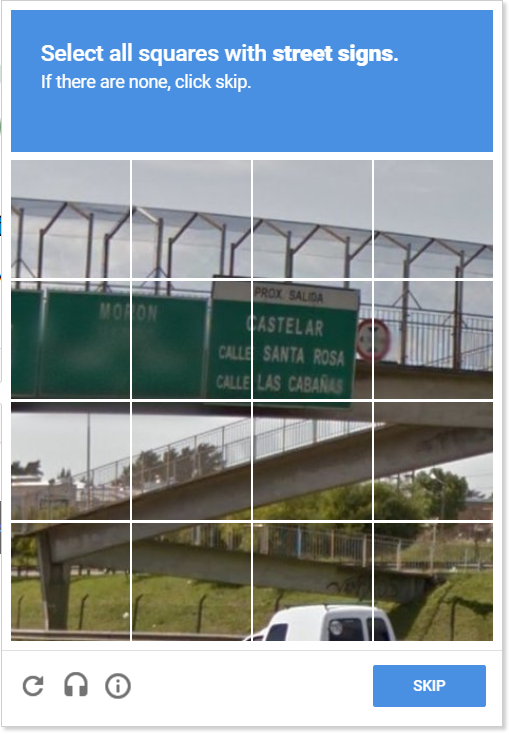
\includegraphics[width=.25\textwidth]{figures/recaptcha.png}
        \framebreak
        \item {\bf Training set:} We need data to train a neural network (e.g.~a MLP).
        \item {\bf Test set:} Once the neural network is trained: \emph{Need to evaluate performance} on another labeled dataset!
        \item {\bf Split the dataset:} Split all labeled data into a subset used for training and its complement used for testing.
        \item {\bf Hyperparameters:} Parameters that determine $\nn$: $L, \{m_l\}_l, \learningrate, \dots$
        \item {\bf Validation set:} Actually, keep a small part of the data set on the side to test different hyperparameters.

        \framebreak
        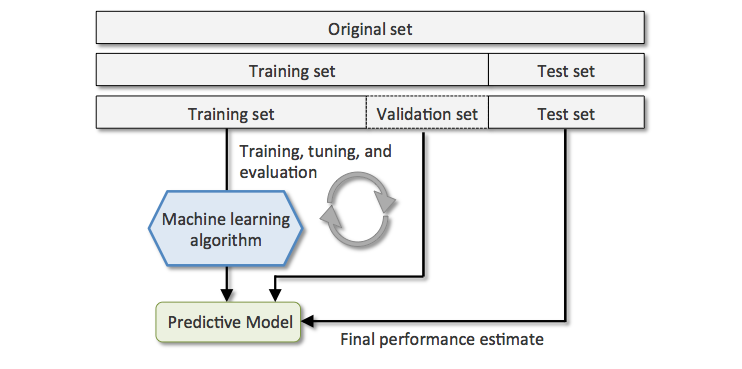
\includegraphics[width=\textwidth]{figures/testtrain.png}
    \end{itemize}
\end{frame}
%%%%%%%%%%%%%%%%%%%%%%%%%%%%%%%%%%%%%%%%%%%
\begin{frame}
    \frametitle{Lab: MLP for digit recognition 2: Training}
        \begin{enumerate}
            \item Define the architecture of the Neural Network.
            \item Load the dataset: Greyscale images are matrices with entries between $0$ (black) and $1$ (dark)\footnote{Actually, images get saved as an array of integers between $0$ an $255$.}.
            \item Split it into Training and Test set.
            \item Visualize some of the elements.
            \item Train the network.
            \item Run a prediction.
            \item Test the accuracy on the test set.
        \end{enumerate}
\end{frame}
%%%%%%%%%%%%%%%%%%%%%%%%%%%%%%%%%%%%%%%%%%%
\begin{frame}
    \frametitle{Optimisers}
        \begin{itemize}
            \item Gradient descent: Easiest to understand, but outperformed by many derived algorithms.
            \item ADAM: \emph{Adaptive moment estimation}:\\
                \begin{enumerate}
                    \item Each iteration on a \emph{random batch} of the dataset.
                    \item Renders gradient a random quantity.
                    \item Estimates the first and second moments of gradient.
                    \item New hyperparameters related to estimation.
                    \item Finds an adaptive learning rate $\learningrate$ in each step.
                \end{enumerate}
            \item
        \end{itemize}
\end{frame}
%%%%%%%%%%%%%%%%%%%%%%%%%%%%%%%%%%%%%%%%%%%
\begin{frame}
    \frametitle{Remarks}
    \begin{itemize}
        %\item {\bf Forward vs.~Backward:}
        %    \begin{itemize}
        %        \item In a forward step, start with input, follow the graph to compute output.
        %        \item In a Gradient Descent step: Compute gradient with respect to parameters starting from output, moving towards input.
        %    \end{itemize}
        \item ``Multilayer Perceptron'' is ``Feed-forward Neural Network''
        \item Do {\bf one} optimization step on {\bf various} samples in one iteration: {\bf Batch size} as hyperparameter.
        \item {\bf Epoch:} Number of times optimizer runs through entire dataset.
        \item The more complex a Neural Network gets, the more complex it can be to compute the gradient.
        \item {\bf Rademacher's Theorem:} If $g^{[l]}$ is \emph{locally Lipschitz continuous}, then it is (Lebesgue-)almost everywhere differentiable, but the the chain rule may not hold everywhere. Generalisations are being developed\footnote{Berner et.al.~\emph{Towards a regularity theory for ReLU networks - Chain rule and global error estimates}. May 2019. \url{https://arxiv.org/pdf/1905.04992.pdf}}.
        \hfill $\Rightarrow$ Many open questions.
    \end{itemize}
\end{frame}
%%%%%%%%%%%%%%%%%%%%%%%%%%%%%%%%%%%%%%%%%%%
\section{Practical remarks}
%%%%%%%%%%%%%%%%%%%%%%%%%%%%%%%%%%%%%%%%%%%
\subsection{Overfitting and Underfitting}
%%%%%%%%%%%%%%%%%%%%%%%%%%%%%%%%%%%%%%%%%%%
\begin{frame}[allowframebreaks]
    \frametitle{Overfitting and Underfitting}
    After training a Neural Network, observe accuracy on training set and on test set.
    \begin{itemize}
        \item If $\nn$ is {\bf inaccurate on the training and test set}
        \begin{itemize}
            \item Model does not capture data (Underfitting).
            \item Model has low variance, high bias.
            \item {\bf Change:} More epochs, bigger training set, more layers, larger layers.
        \end{itemize}
        \item If $\nn$ is {\bf accurate on the training set, inaccurate on test set}
        \begin{itemize}
            \item Model interpolates training data, extrapolates poorly: {\bf Overfitting}
            \item Model has high variance, low bias.
            \item {\bf Change:} Fewer epochs, smaller training set, smaller $\nn$.
        \end{itemize}
    \framebreak
    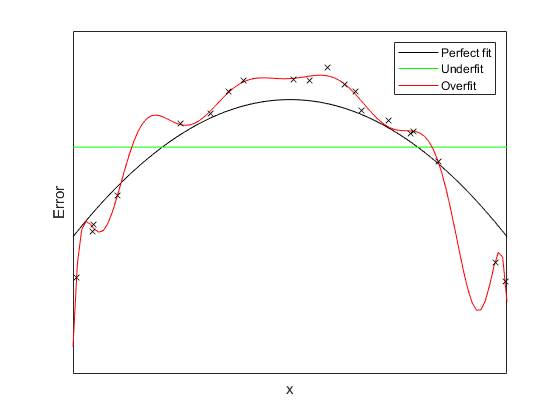
\includegraphics[width=.9\textwidth]{figures/overunder1.png}
    \framebreak
    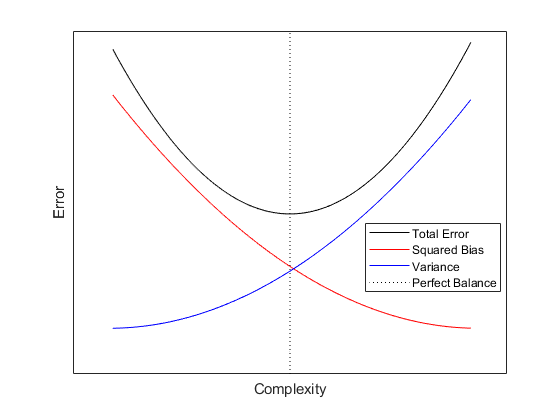
\includegraphics[width=.9\textwidth]{figures/overunder2.png}
    \framebreak
    \item {\bf Regularization:}

    \begin{itemize}
        \item Replace $\loss(\nn; \dataset)$ by
        $$
            \loss(\nn; \dataset) + \lambda \operatorname{Reg}(\nn)
            \;,
        $$
        where
        $$
            \operatorname{Reg}(\nn) := \frac{1}{L} \sum_{l=0}^L\left\|W^{[l, l+1]}\right\|^2
            \;.
        $$
        Common to choose the Frobenius Norm.
        \item Penalise large weights $\Rightarrow$ scaled input for activation.
        \item {\bf New hyperparameter} $\lambda$.
        \item {\tt PyTorch:} Parameter {\tt weight\_decay} in {\tt optimizer}.
    \end{itemize}
    \framebreak
    \item {\bf Dropout:}

        \begin{itemize}
            \item {\bf During training}, randomly deactivate some neurons.
            \item Choose a dropout probability $p_d \in [0,1)$.
            \item During training, each neuron will be multiplied by $0$ with probability $p_d$.
            \item ``Decrease the influence of single neurons on the output of $\nn$.''
            \item {\tt PyTorch}: Before training, set {\tt model.eval()} to deactivate dropout.
        \end{itemize}
    \end{itemize}
\end{frame}
%%%%%%%%%%%%%%%%%%%%%%%%%%%%%%%%%%%%%%%%%%%
\begin{frame}[allowframebreaks]
    \frametitle{Initialisation}
    \begin{itemize}
        \item Optimisation: $
            \boldsymbol{\xi}^{\text{new}} := \boldsymbol{\xi}^{\text{current}}
            - \learningrate \nabla_{\boldsymbol{\xi}}J(\boldsymbol{\xi}^{\text{current}};\dataset)$
        \item Initial value needed.
        \item What happens if we initialise all weights to $0$?\\

        \begin{tikzpicture}[shorten >=1pt,->,draw=black!50, node distance=\layersep]
    \tikzstyle{every pin edge}=[<-,shorten <=1pt]
    \tikzstyle{neuron}=[circle,fill=black!25,minimum size=17pt,inner sep=0pt]
    \tikzstyle{input neuron}=[neuron, fill=green!50];
    \tikzstyle{output neuron}=[neuron, fill=red!50];
    \tikzstyle{hidden neuron}=[neuron, fill=blue!50];
    \tikzstyle{annot} = [text width=4em, text centered]

    % Draw the input layer nodes
    \foreach \name / \y in {1,...,3}
    % This is the same as writing \foreach \name / \y in {1/1,2/2,3/3,4/4}
        \node[input neuron] (I-\name) at (0,-\y) {$x_{\y}$};

    % Draw the hidden layer nodes
    \foreach \name / \y in {1,...,4}
        \path[yshift=0.5cm]
            node[hidden neuron] (H1-\name) at (\layersep,-\y cm) {$h^{[1]}_{\y}$};

    % Draw the hidden layer nodes
    \foreach \name / \y in {1,...,4}
        \path[yshift=0.5cm]
            node[hidden neuron, right of=H1-\name] (Hdots-\name) at (\layersep,-\y cm) {$\dots$};


    % Draw the hidden layer nodes
    \foreach \name / \y in {1,...,3}
        \path[yshift=0.5cm]
            node[hidden neuron, right of=Hdots-\name] (H2-\name) {$h^{[L]}_{\y}$};

    % Draw the output layer node
    \node[output neuron, right of=H2-3] (O) {$y$};

    % Connect every node in the input layer with every node in the
    % hidden layer.
    \foreach \source in {1,...,3}
        \foreach \dest in {1,...,4}
            \path (I-\source) edge (H1-\dest);

    \foreach \source in {1,...,4}
        \foreach \dest in {1,...,4}
            \path (H1-\source) edge (Hdots-\dest);

    % Connect every node in the first hidden layer with every node in the
    % hidden layer 2.
    \foreach \source in {1,...,4}
        \foreach \dest in {1,...,3}
            \path (Hdots-\source) edge (H2-\dest);

    % Connect every node in the hidden layer with the output layer
    \foreach \source in {1,...,3}
        \path (H2-\source) edge (O);
\end{tikzpicture}

        \framebreak
        \item {\bf Random initialisation:} Draw initial parameters from probability distribution (uniform, normal).
        \item What happens if the initial values are around zero?
        \item What happens if the initial values are large in absolute value?
        \item {\bf Idea:} For $W^{[l, l+1]}$, decrease variance with $m_l$ to ensure that weights get iterated differently.
        \item {\bf Xavier initialisation\footnote{Glorot and Bengio: \emph{Understanding the difficulty of training deep feedforward neural networks.}, 2010.}:} Initialisation of $W^{[l, l+1]}$ by unform distribution around $0$ with standard deviation $\frac{1}{m_{l}}$.\\[.5em]
        Works well with $\tanh$, $\sigma$ activations.
        \item {\bf He initialisation\footnote{He et al.: \emph{Delving Deep into Rectifiers: Surpassing Human-Level Performance on ImageNet Classification.}, 2015.}:} Initialisation of $W^{[l, l+1]}, b^{[l, l+1]}$ by $\mathcal{N}\left(0, \frac{1}{m_{l}}\right)$.\\
        Works well with $\relu$ and
        $$
            \prelu_{\beta}(x):=\max(-\beta x, x)
            \;,\qquad
            \text{(typically, $0<\beta<<1$)}
            \;.
        $$
    \end{itemize}
\end{frame}
%%%%%%%%%%%%%%%%%%%%%%%%%%%%%%%%%%%%%%%%%%%
\begin{frame}
    \frametitle{Deep vs.~Shallow}
    \begin{itemize}
        \item Adding more layers vs.~enlarging present layers: Adding more features vs.~combining present features.
        \item \emph{Deep} layers ($h^{[l]}$ for large $l$) learn more complex features.
    \end{itemize}
    \begin{theorem}[Approximation properties of Neural Networks (Sketch)]
        \begin{enumerate}
            \setcounter{enumi}{-1}
            \item Given a function $f\in C^{(0,1)}(\Omega)$ to be approximated by $\nn$, $\Omega\in\R^{m_0}$ compact.
            \item Both shallow (small fixed $L$) and deep (large $L$) NN can compute the best approximation of $f$ in finitely many steps.
            \item Let $M$ be complexity needed to surely attain accuracy $\varepsilon>0$.
                \begin{itemize}
                    \item If $L=1$, need to increase $m_1$ \emph{exponentially} to attain $\varepsilon>0$.
                    \item In the deep case, it is sufficient to increase $L$ at most \emph{linearly}.
                    \item Depends on \emph{complexity} of $f$: ``How many compositions are needed to express $f$ in elementary functions?''
                \end{itemize}
        \end{enumerate}
    \end{theorem}
\end{frame}
%%%%%%%%%%%%%%%%%%%%%%%%%%%%%%%%%%%%%%%%%%%
\begin{frame}
    \frametitle{Recapitulation: Neural Networks}
    \begin{enumerate}
        \item A Neural Network (MLP) $\nn$ contains a forward step (prediction) and a backward step (learning).
        \item {\bf Forward step:} Composition of affine maps and activation functions, using learned parameters.
        \item {\bf Backward step:} Optimization (``learning'') of parameters to minimise a \emph{loss function} $\loss(\nn; \dataset)$.
        \item {\bf Initialisation:} Find ``smart'' way to initialise minimisation.
        \item {\bf Train/Test set:} $\dataset=\dataset_{\text{train}}\dot{\cup} \dataset_{\text{test}}$, usually $\frac{\left|\dataset_{\text{train}}\right|}{\left|\dataset\right|} \in [0.6, 0.9]$.
        \item {\bf Bias-Variance tradeoff:} $\nn$ needs to fit the data \emph{reasonably} well, but still extrapolate on unknown data.
        \item {\bf ``Magic'':} Many heuristic tweaks.
        \item ``Deep'': $L\simeq$``depth'' of $\nn$. The deeper the network, the more complex the learned features.
    \end{enumerate}
\end{frame}
%%%%%%%%%%%%%%%%%%%%%%%%%%%%%%%%%%%%%%%%%%%
\section{CNNs}
\subsection{Convolutional layers}
%%%%%%%%%%%%%%%%%%%%%%%%%%%%%%%%%%%%%%%%%%%
\begin{frame}[allowframebreaks]
    \frametitle{Convolutional Layers}
    \begin{itemize}
        \item Before: Each layer is $g^{[l]}$ of a linear combination of $h^{[l-1]}$: {\bf Fully connected layers}.
        \item Introduce new kinds of layers for image processing.
        \item {\bf Motivation:} Visual computing.
        \item {\bf Image input:} $n_x \times n_y$ pixels, $n_c$ channels: $m_0=n_xn_yn_c$!
        \item {\bf Idea:} To obtain a sense of vicinity: Go through each pixel and combine only its surrounding pixels linearly.
        \item To maximize confusion, what we call convolution here is actually a cross-correlation. Difference: Transposition of the filter.
        \framebreak
        \item {\bf Convolution with a filter:}\\

        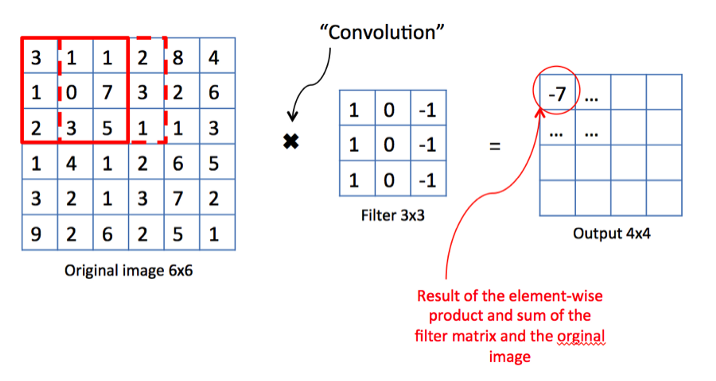
\includegraphics[width=.8\textwidth]{figures/convlayer.png}

        \item
        This is an example of a {\bf vertical edge detector}: If the resulting number is large, it means that the pixel values to the left and to the right are different.
        \framebreak
        \item Classical Edge detection: Design such filters for each use case (Sobel, Laplace, Scharr, ...)
        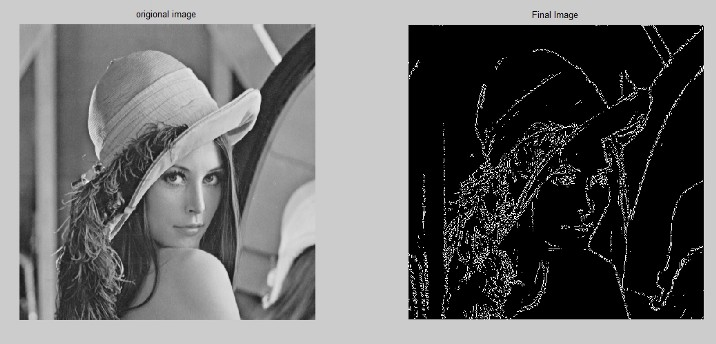
\includegraphics[width=.8\textwidth]{figures/sobel.jpg}
        \item {\bf Convolutional layer:} One layer consists of $m_l$ filters. The entries of the filters are \emph{learned}.
        \item Resulting size: Image size $n\times n$, Filter size $f\times f$: Results in output size $(n-f+1)\times (n-f+1)$.
    \end{itemize}
\end{frame}
%%%%%%%%%%%%%%%%%%%%%%%%%%%%%%%%%%%%%%%%%%%
\begin{frame}
    \frametitle{Padding}
    \begin{itemize}
        \item {\bf Problem:} Each time a filter is applied, image size decreases.
        \item {\bf Padding:} Embed the image inside an outer layer of zeroes.
        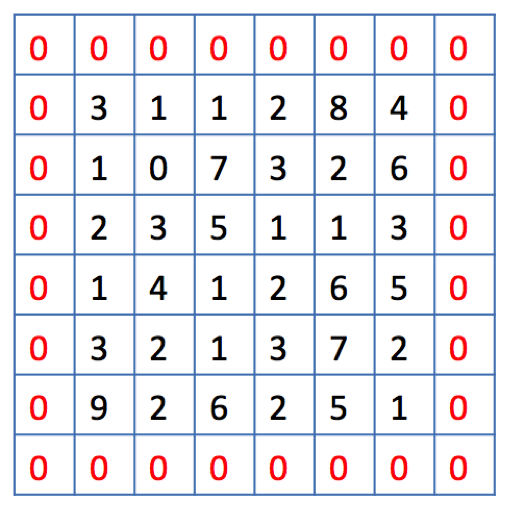
\includegraphics[width=.3\textwidth]{figures/padding.png}
        \item Resulting output size with padding $p$, input size $n$, filter size $f$:  $(n+2p-f+1)\times (n+2p-f+1)$.
        \item Enforce input size$=$output size by $p=\frac{f-1}{2}$.
        \item Therefore filter sizes are usually odd numbers.
    \end{itemize}
\end{frame}
%%%%%%%%%%%%%%%%%%%%%%%%%%%%%%%%%%%%%%%%%%%
\begin{frame}
    \frametitle{Strided convolution}
    \begin{itemize}
        \item So far:
        \begin{enumerate}
            \item Apply a filter to pixel $(i,j)$ in input to get pixel $(k,l)$ in output.
            \item Apply a filter to pixel $(i+1,j)$ in input to get pixel $(k+1,l)$ in output.
        \end{enumerate}
        \item With {\bf stride} $s$:
        \begin{enumerate}
            \item Apply a filter to pixel $(i,j)$ in input to get pixel $(k,l)$ in output.
            \item Apply a filter to pixel $(i+{\color{red}s},j)$ in input to get pixel $(k+1,l)$ in output.
        \end{enumerate}
        \item Output size: $\left\lfloor\frac{n+2p-f}{s}+1\right\rfloor\times \left\lfloor\frac{n+2p-f}{s}+1\right\rfloor$
    \end{itemize}
\end{frame}
%%%%%%%%%%%%%%%%%%%%%%%%%%%%%%%%%%%%%%%%%%%
\begin{frame}
    \frametitle{Recap: Convolutional Layers}
    \begin{itemize}
        \item A {\bf convolutional layer} applies a filter to an output to detect a feature.
        \item What kind of filter yields the best classification results will be learned.
        \item To ensure more flexibility, a convolutional layer has hyperparameters {\bf Filter size, Padding, Stride}.
        \item Usually followed by $\relu$ activation function.
    \end{itemize}
\end{frame}
%%%%%%%%%%%%%%%%%%%%%%%%%%%%%%%%%%%%%%%%%%%
\begin{frame}[allowframebreaks]
    \frametitle{Pooling layer}
    \begin{itemize}
        \item Convolution can result in large output image, features too detailed.
        \item {\bf Idea:} Generate a ``summary'' of the different areas in the image.
        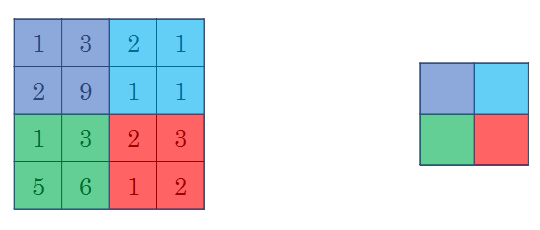
\includegraphics[width=.5\textwidth]{figures/pooling1.png}
        \item Most common: {\bf Max-pooling}.
        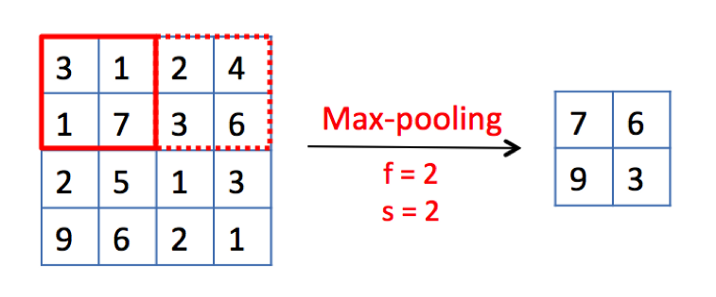
\includegraphics[width=.5\textwidth]{figures/pooling2.png}
        \framebreak
        \item Hyperparameters: filter size, stride, kind of pooling.
        \item Introduces more flexibility on output size.
        \item Reduces output to relevant features.
        \item Therefore usually combined with $\relu$.
        \item Considered as part of the convolutional layer.
    \end{itemize}
\end{frame}
%%%%%%%%%%%%%%%%%%%%%%%%%%%%%%%%%%%%%%%%%%%
\begin{frame}[allowframebreaks]
    \frametitle{A typical CNN architecture: VGG-16}
    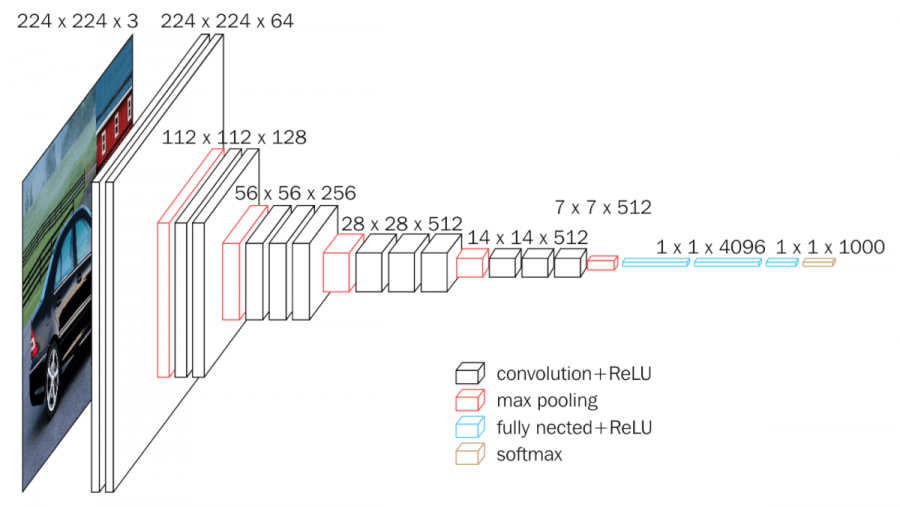
\includegraphics[width=.9\textwidth]{figures/vgg16.png}
    \framebreak
    \begin{itemize}
        \item Developed by the {\bf V}isual {\bf C}omputing {\bf G}roup in Oxford\footnote{Simonyan and Zisserman: \emph{Very Deep Convolutional Networks for Large-Scale Image Recognition.} 2015}
        \item VGG-16 classifies for $1000$ objects on an image.
        \item Image size decreases while number of filters increases.
        \item Backpropagation now involves derivatives w.r.~to the new parameters.
        \item Convolutional Layers learn ``$m_l$'' filters: {\bf Feature maps}
        \begin{tikzpicture}
%\node at (1.5,4){\begin{tabular}{c}input image\\or input feature map\end{tabular}};

\draw (0,0) -- (3,0) -- (3,3) -- (0,3) -- (0,0);

\draw (2,2) -- (2.5,2) -- (2.5,2.5) -- (2,2.5) -- (2,2);
\draw (2,0.5) -- (2.5,0.5) -- (2.5,1) -- (2,1) -- (2,0.5);
\draw (1,1) -- (1.5,1) -- (1.5,1.5) -- (1,1.5) -- (1,1);

\draw (2.5,2) -- (7,3.25);
\draw (2.5,2.5) -- (7,3.25);

\draw (2.5,1) -- (5.75,0.25);
\draw (2.5,0.5) -- (5.75,0.25);

\draw (1.5,1.5) -- (5.5,1.25);
\draw (1.5,1) -- (5.5,1.25);

%\node at (5.75,4){\begin{tabular}{c}output feature maps\end{tabular}};

\draw[fill=black,opacity=0.2,draw=black] (5.5,1.5) -- (7.5,1.5) -- (7.5,3.5) -- (5.5,3.5) -- (5.5,1.5);
\draw[fill=black,opacity=0.2,draw=black] (5,1) -- (7,1) -- (7,3) -- (5,3) -- (5,1);
\draw[fill=black,opacity=0.2,draw=black] (4.5,0.5) -- (6.5,0.5) -- (6.5,2.5) -- (4.5,2.5) -- (4.5,0.5);
\draw[fill=black,opacity=0.2,draw=black] (4,0) -- (6,0) -- (6,2) -- (4,2) -- (4,0);
\end{tikzpicture}

    \end{itemize}
\end{frame}
%%%%%%%%%%%%%%%%%%%%%%%%%%%%%%%%%%%%%%%%%%%
\section{Style Transfer}
\subsection{Lab: Visualisation of Neurons}
%%%%%%%%%%%%%%%%%%%%%%%%%%%%%%%%%%%%%%%%%%%
\begin{frame}
    \frametitle{Lab: Visualisation of Neurons}
    \begin{itemize}
        \item Lower layers learn simple features: Edges, curves, repetitive patterns.
        \item Higher layers learn complex features, distinguishing very similar outputs (cat ears, dog ears, eyes,...)
        \item Visualization of the filters contained in one layer:
        \begin{enumerate}
            \item Start with a random image.
            \item Choose a neuron $f_{k}^{[l]}$: Filter $k$ in layer $l$.
            \item {\bf Modify the image to maximize the activation of $f_{k}^{[l]}$}.
            \item Display the resulting image.
        \end{enumerate}
    \end{itemize}
\end{frame}
%%%%%%%%%%%%%%%%%%%%%%%%%%%%%%%%%%%%%%%%%%%
\subsection{Lab: Style transfer learning}
%%%%%%%%%%%%%%%%%%%%%%%%%%%%%%%%%%%%%%%%%%%
\begin{frame}[allowframebreaks]
    \frametitle{Lab: Style transfer learning}
    \begin{itemize}
        \item Given one image $I_s$ as a style template and one image $I_c$ as a content template.
        \item {\bf Goal:} Create an image of the content of $I_c$, but in the style of $I_s$.
        \framebreak
        \item {\bf Style transfer learning:} Use a trained Neural Network to measure \emph{difference in style} and \emph{difference in content}.
        \begin{enumerate}
            \item Load a pre-trained Convolutional Network.
            \item Identify layers and neurons (filters) corresponding to \emph{style} and \emph{content}. \\
            Their output define a content loss and a style loss:
            $$
                \loss_{\text{content}}(I, I_c) = \|\operatorname{content}(I)-\operatorname{content}(I_c)\|^2\;,
            $$
            analogously with style loss.\\
            Total variation loss: Combination of style and content loss, plus regularization.
            \item Start with randomised image and iterate the pixel values to minimize Total variation loss.
        \end{enumerate}
    \end{itemize}
\end{frame}
\begin{frame}
    \frametitle{Style Transfer: Results}
    \centering
    \only<1>{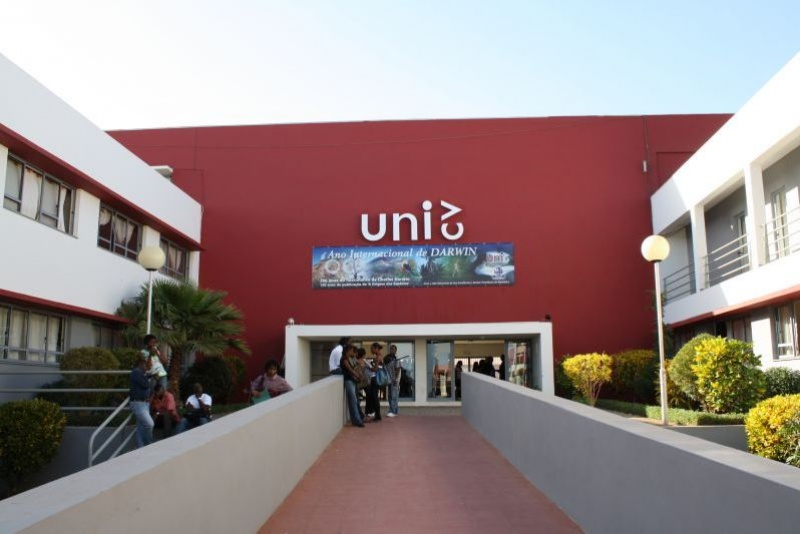
\includegraphics[width=.9\textwidth]{figures/unicv.jpg}}
    \only<2>{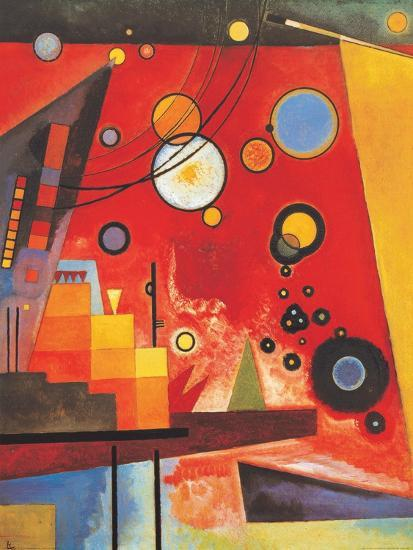
\includegraphics[height=.8\textheight]{figures/kandinsky2.jpg}
            \\{\small \emph{``Heavy Red''}, Kandinskiy 1924}}
    \only<3>{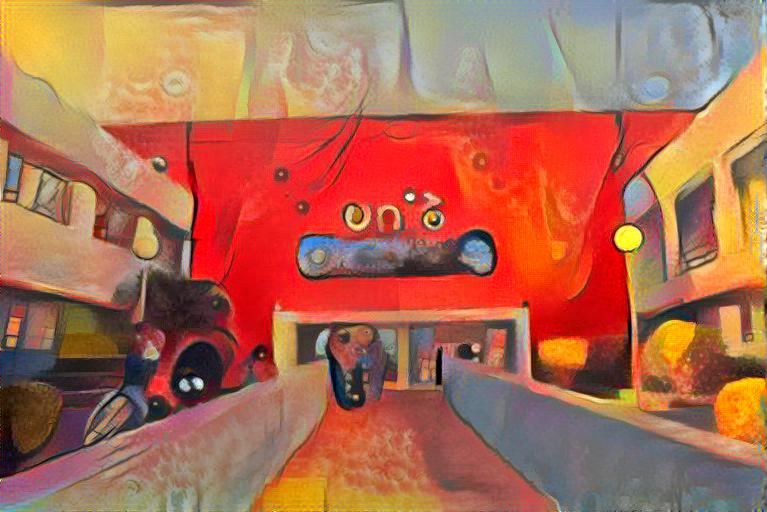
\includegraphics[width=.9\textwidth]{figures/out_unicv_kandinsky.jpg}
    \\{\small \emph{``University of Cape Verde''}, Kandinskiy 2019}}
    \only<4>{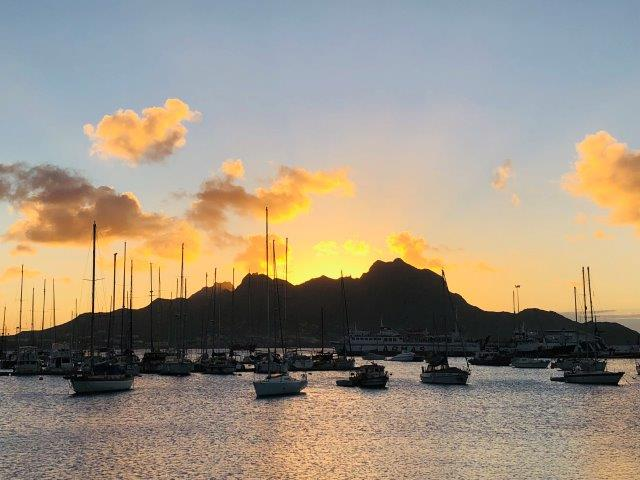
\includegraphics[height=.8\textheight]{figures/mindelo.jpg}}
    \only<5>{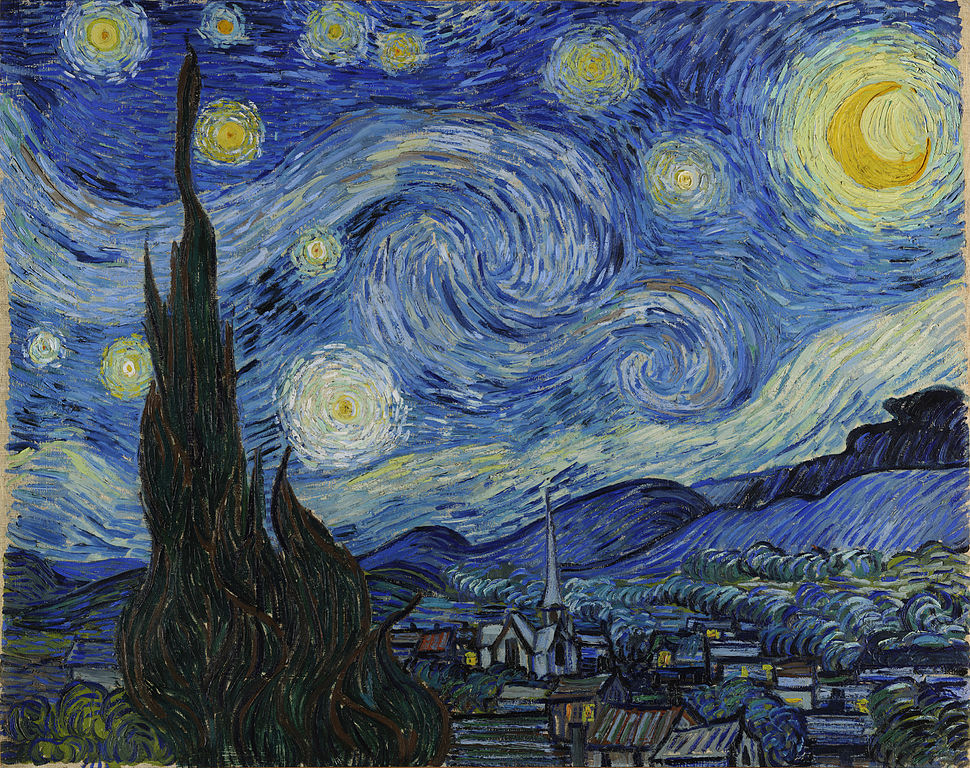
\includegraphics[width=.8\textwidth]{figures/starrynight.jpg}
            \\{\small \emph{``Starry Night''}, Van Gogh 1889}}
    \only<6>{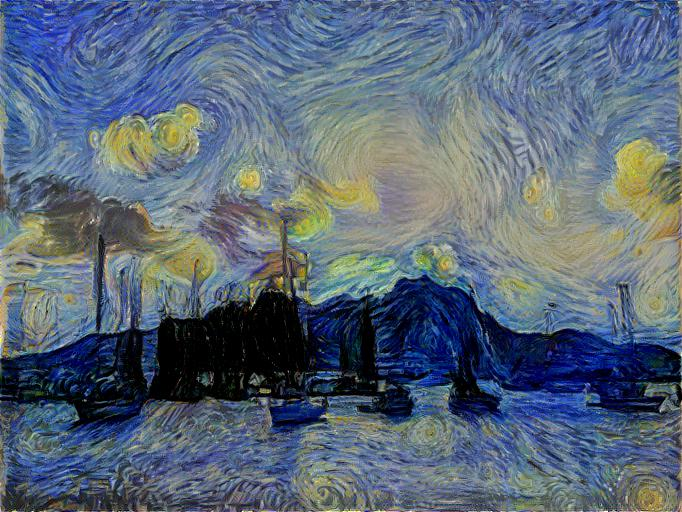
\includegraphics[width=.8\textwidth]{figures/out_mindelo_starrynight.jpg}
    \\{\small \emph{``Starry Monte Cara''}, Van Gogh 2019}}
    \only<7>{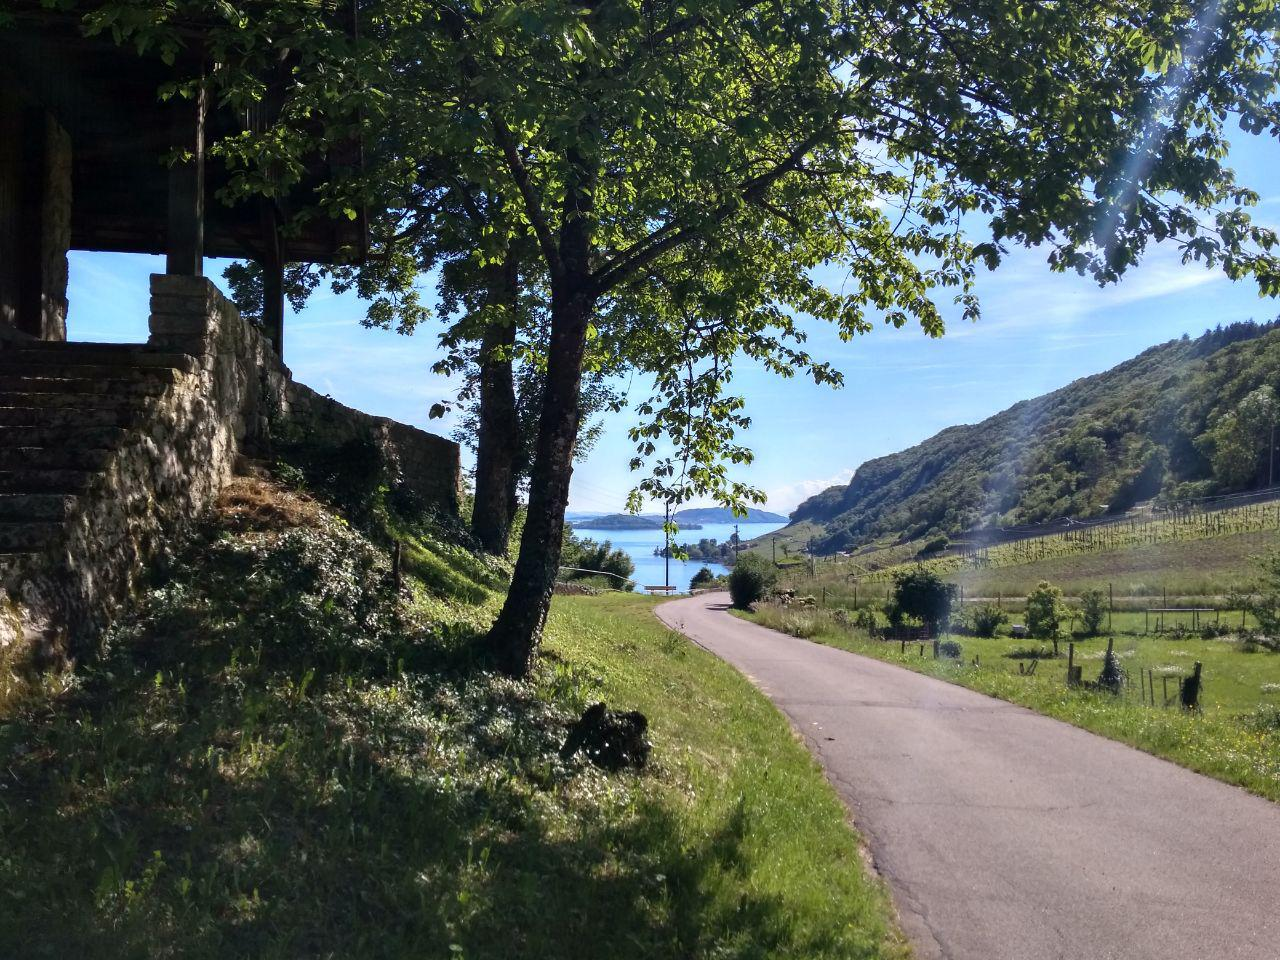
\includegraphics[height=.8\textheight]{figures/weinberg_orig.jpg}}
    \only<8>{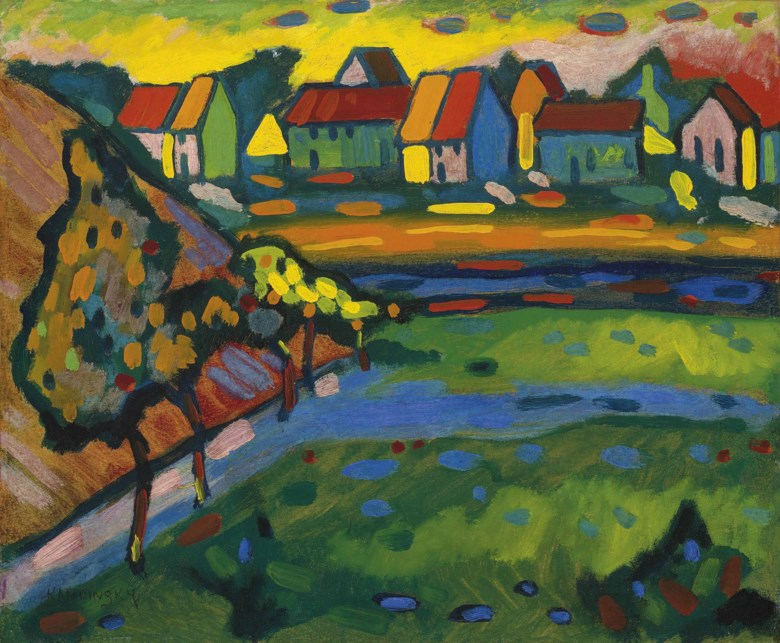
\includegraphics[width=.8\textwidth]{figures/kandinsky3.jpg}
            \\{\small \emph{``Bavarian Village''}, Kandinskiy 1908}}
    \only<9>{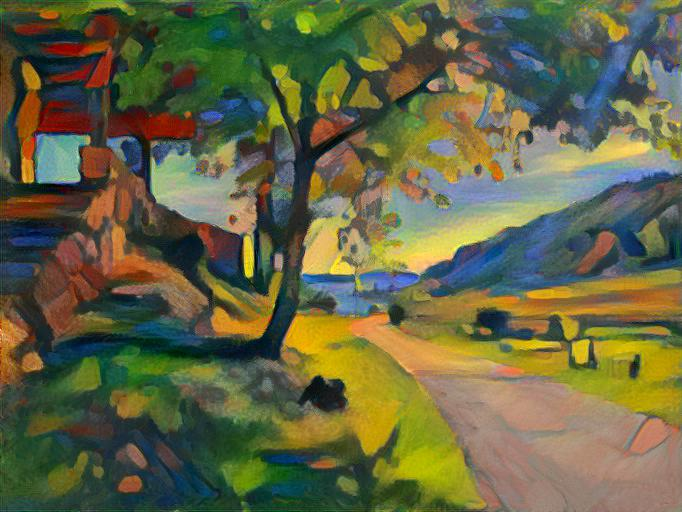
\includegraphics[width=.8\textwidth]{figures/out_weinberg_kandinsky3.jpg}
    \\{\small \emph{``Lake Biel''}, Kandinskiy 2019}}
\end{frame}
%%%%%%%%%%%%%%%%%%%%%%%%%%%%%%%%%%%%%%%%%%%
\begin{frame}
    \frametitle{Some things left out}
    \begin{itemize}
        \item {\bf Data augmentation:} How to get more out of a dataset.
        \item {\bf Data normalization:} How to scale the input to increase learning performance.
        \item {\bf Exploding gradients:} Really large $L$ imply instabilities of gradients.
        \item {\bf Image segmentation} vs.~classification.
        \item Recurrent Neural Networks (RNNs), Residual Networks, Generative Adversarial Networks, U-Nets, ...
        \item {\bf RNNs:} If your data is \emph{sequential} (e.g.~Time series, Music, Natural Language), there is a type of neuron that learns to predict the next value: \emph{Long short-term memory cells} (LSTM).
    \end{itemize}
\end{frame}
%%%%%%%%%%%%%%%%%%%%%%%%%%%%%%%%%%%%%%%%%%%
\begin{frame}
    \frametitle{Thank you.}
    \centering {\bf Thank you for your attention and your hospitality!}
\end{frame}

\end{document}
